\documentclass[10pt,a4paper,twoside]{report}

% ----------------------------------------------------------------------
% Define external packages, language, margins, fonts and new commands
% ----------------------------------------------------------------------
% ----------------------------------------------------------------------
% Define document language.
% ----------------------------------------------------------------------

% 'inputenc' package
%
% Accept different input encodings.
% http://www.ctan.org/tex-archive/macros/latex/base/
%
% > allows typing non-english text in LaTeX sources.
%
% ******************************* SELECT *******************************
%\usepackage[latin1]{inputenc} % <<<<< Windows
\usepackage[utf8]{inputenc}   % <<<<< Linux
% ******************************* SELECT *******************************

% 'comments' package
% verbatim
\usepackage{verbatim}


% 'babel' package
%
% Multilingual support for Plain TeX or LaTeX.
% http://www.ctan.org/tex-archive/macros/latex/required/babel/
%
% > sets the variable names according to the language selected
%
% ******************************* SELECT *******************************
%\usepackage[portuguese]{babel} % <<<<< Portuguese
\usepackage[english]{babel} % <<<<< English
% ******************************* SELECT *******************************


% List of LaTeX variable names: \abstractname, \appendixname, \bibname,
%   \chaptername, \contentsname, \listfigurename, \listtablename, ...)
% http://www.tex.ac.uk/cgi-bin/texfaq2html?label=fixnam
%
% Changing the words babel uses (uncomment and redefine as necessary...)
%
\newcommand{\acknowledgments}{@undefined} % new LaTeX variable name
%
% > English
%
\addto\captionsenglish{\renewcommand{\acknowledgments}{Acknowledgments}}
%\addto\captionsenglish{\renewcommand{\contentsname}{Contents}}
%\addto\captionsenglish{\renewcommand{\listtablename}{List of Tables}}
%\addto\captionsenglish{\renewcommand{\listfigurename}{List of Figures}}
%\addto\captionsenglish{\renewcommand{\nomname}{Nomenclature}}
%\addto\captionsenglish{\renewcommand{\glossaryname}{Glossary}}
%\addto\captionsenglish{\renewcommand{\acronymname}{List of Acronyms}}
%\addto\captionsenglish{\renewcommand{\bibname}{References}} % Bibliography
%\addto\captionsenglish{\renewcommand{\appendixname}{Appendix}}

% > Portuguese
%
\addto\captionsportuguese{\renewcommand{\acknowledgments}{Agradecimentos}}
%\addto\captionsportuguese{\renewcommand{\contentsname}{Conte\'{u}do}}
%\addto\captionsportuguese{\renewcommand{\listtablename}{Lista de Figuras}}
%\addto\captionsportuguese{\renewcommand{\listfigurename}{Lista de Tabelas}}
\addto\captionsportuguese{\renewcommand{\nomname}{Lista de S\'{i}mbolos}} % Nomenclatura
%\addto\captionsportuguese{\renewcommand{\glossary}{Gloss\'{a}rio}}
%\addto\captionsportuguese{\renewcommand{\acronymname}{Lista de Abrevia\c{c}\~{o}es}}
%\addto\captionsportuguese{\renewcommand{\bibname}{Refer\^{e}ncias}} % Bibliografia
%\addto\captionsportuguese{\renewcommand{\appendixname}{Anexo}} % Apendice


% ----------------------------------------------------------------------
% Define cover fields in both english and portuguese.
% ----------------------------------------------------------------------
%
\newcommand{\coverThesis}{@undefined} % new LaTeX variable name
\newcommand{\coverSupervisors}{@undefined} % new LaTeX variable name
\newcommand{\coverExaminationCommittee}{@undefined} % new LaTeX variable name
\newcommand{\coverChairperson}{@undefined} % new LaTeX variable name
\newcommand{\coverSupervisor}{@undefined} % new LaTeX variable name
\newcommand{\coverMemberCommittee}{@undefined} % new LaTeX variable name
% > English
\addto\captionsenglish{\renewcommand{\coverThesis}{Thesis to obtain the Master of Science Degree in}}
\addto\captionsenglish{\renewcommand{\coverSupervisors}{Supervisor(s)}}
\addto\captionsenglish{\renewcommand{\coverExaminationCommittee}{Examination Committee}}
\addto\captionsenglish{\renewcommand{\coverChairperson}{Chairperson}}
\addto\captionsenglish{\renewcommand{\coverSupervisor}{Supervisor}}
\addto\captionsenglish{\renewcommand{\coverMemberCommittee}{Member of the Committee}}
% > Portuguese
\addto\captionsportuguese{\renewcommand{\coverThesis}{Disserta\c{c}\~{a}o para obten\c{c}\~{a}o do Grau de Mestre em}}
\addto\captionsportuguese{\renewcommand{\coverSupervisors}{Orientador(es)}}
\addto\captionsportuguese{\renewcommand{\coverExaminationCommittee}{J\'{u}ri}}
\addto\captionsportuguese{\renewcommand{\coverChairperson}{Presidente}}
\addto\captionsportuguese{\renewcommand{\coverSupervisor}{Orientador}}
\addto\captionsportuguese{\renewcommand{\coverMemberCommittee}{Vogal}}


% ----------------------------------------------------------------------
% Define default and cover page fonts.
% ----------------------------------------------------------------------

% Use Arial font as default
%
\renewcommand{\rmdefault}{phv}
\renewcommand{\sfdefault}{phv}

% Define cover page fonts
%
%         encoding     family       series      shape
%  \usefont{T1}     {phv}=helvetica  {b}=bold    {n}=normal
%                   {ptm}=times      {m}=normal  {sl}=slanted
%                                                {it}=italic
% see more examples at
% http://julien.coron.free.fr/languages/latex/fonts/
%
\def\FontLn{% 16 pt normal
  \usefont{T1}{phv}{m}{n}\fontsize{16pt}{16pt}\selectfont}
\def\FontLb{% 16 pt bold
  \usefont{T1}{phv}{b}{n}\fontsize{16pt}{16pt}\selectfont}
\def\FontMn{% 14 pt normal
  \usefont{T1}{phv}{m}{n}\fontsize{14pt}{14pt}\selectfont}
\def\FontMb{% 14 pt bold
  \usefont{T1}{phv}{b}{n}\fontsize{14pt}{14pt}\selectfont}
\def\FontSn{% 12 pt normal
  \usefont{T1}{phv}{m}{n}\fontsize{12pt}{12pt}\selectfont}


% ----------------------------------------------------------------------
% Define page margins and line spacing.
% ----------------------------------------------------------------------

% 'geometry' package
%
% Flexible and complete interface to document dimensions.
% http://www.ctan.org/tex-archive/macros/latex/contrib/geometry/
%
% > set the page margins (2.5cm minimum in every side, as per IST rules)
%
\usepackage{geometry}	
\geometry{verbose,tmargin=2.5cm,bmargin=2.5cm,lmargin=2.5cm,rmargin=2.5cm}

% 'setspace' package
%
% Set space between lines.
% http://www.ctan.org/tex-archive/macros/latex/contrib/setspace/
%
% > allow setting line spacing (line spacing of 1.5, as per IST rules)
%
\usepackage{setspace}
\renewcommand{\baselinestretch}{1.5}


% ----------------------------------------------------------------------
% Include external packages.
% Note that not all of these packages may be available on all system
% installations. If necessary, include the .sty files locally in
% the <jobname>.tex file directory.
% ----------------------------------------------------------------------

% 'graphicx' package
%
% Enhanced support for graphics.
% http://www.ctan.org/tex-archive/macros/latex/required/graphics/
%
% > extends arguments of the \includegraphics command
%
\usepackage{graphicx}


% 'color' package
%
% Colour control for LaTeX documents.
% http://www.ctan.org/tex-archive/macros/latex/required/graphics/
%
% > defines color macros: \color{<color name>}
%
%\usepackage{color}


% 'amsmath' package
%
% Mathematical enhancements for LaTeX.
% http://www.ctan.org/tex-archive/macros/latex/required/amslatex/
%
% > American Mathematical Society plain Tex macros
%
\usepackage{amsmath}  % AMS mathematical facilities for LaTeX.
\usepackage{amsthm}   % Typesetting theorems (AMS style).
\usepackage{amsfonts} % 


% 'wrapfig' package
%
% Produces figures which text can flow around.
% http://www.ctan.org/tex-archive/macros/latex/contrib/wrapfig/
%
% > wrap figures/tables in text (i.e., Di Vinci style)
%
% \usepackage{wrapfig}


% 'subfigure' package
%
% Deprecated: Figures divided into subfigures.
% http://www.ctan.org/tex-archive/obsolete/macros/latex/contrib/subfigure/
%
% > subcaptions for subfigures
%
\usepackage{subfigure}


% 'subfigmat' package
%
% Automates layout when using the subfigure package.
% http://www.ctan.org/tex-archive/macros/latex/contrib/subfigmat/
%
% > matrices of similar subfigures
%
\usepackage{subfigmat}


% 'url' package
%
% Verbatim with URL-sensitive line breaks.
% http://www.ctan.org/tex-archive/macros/latex/contrib/url/
%
% > URLs in BibTex
%
% \usepackage{url}


% 'varioref' package
%
% Intelligent page references.
% http://www.ctan.org/tex-archive/macros/latex/required/tools/
%
% > smart page, figure, table and equation referencing
%
%\usepackage{varioref}


% 'dcolumn' package
%
% Align on the decimal point of numbers in tabular columns.
% http://www.ctan.org/tex-archive/macros/latex/required/tools/
%
% > decimal-aligned tabular math columns
%
\usepackage{dcolumn}
\newcolumntype{d}{D{.}{.}{-1}} % column aligned by the point separator '.'
\newcolumntype{e}{D{E}{E}{-1}} % column aligned by the exponent 'E'


% '' package
%
% Reimplementation of and extensions to LaTeX verbatim.
% http://www.ctan.org/tex-archive/macros/latex/required/tools/
%
% > provides the verbatim environment (\begin{verbatim},\end{verbatim})
%   and a comment environment (\begin{comment},  \end{comment})
%
% \usepackage{verbatim}


% 'moreverb' package
%
% Extended verbatim.
% http://www.ctan.org/tex-archive/macros/latex/contrib/moreverb/
%
% > supports tab expansion and line numbering
%
% \usepackage{moreverb}


%%%%%%%%%%%%%%%%%%%%%%%%%%%%%%%%%%%%%%%%%%%%%%%%%%%%%
%           Glossaries & Acronyms
% tools>commands>makeglossaries  
%\newglossaryentry ou \newacronym no fim \printglossaries
%
\usepackage[acronym]{glossaries}
\makeglossaries

%%%%%%%%%%%%%%%%%%%%%%%%%%%%%%%%%%%%%%%%%%%%%%%%%%%%%


% 'nomencl' package
%
% Produce lists of symbols as in nomenclature.
% http://www.ctan.org/tex-archive/macros/latex/contrib/nomencl/
%
% The nomencl package makes use of the MakeIndex program
% in order to produce the nomenclature list.
%
% Nomenclature
% 1) On running the file through LATEX, the command \makenomenclature
%    in the preamble instructs it to create/open the nomenclature file
%    <jobname>.nlo corresponding to the LATEX file <jobname>.tex and
%    writes the information from the \nomenclature commands to this file.
% 2) The next step is to invoke MakeIndex in order to produce the
%    <jobname>.nls file. This can be achieved by making use of the
%    command: makeindex <jobname>.nlo -s nomencl.ist -o <jobname>.nls
% 3) The last step is to invoke LATEX on the <jobname>.tex file once
%    more. There, the \printnomenclature in the document will input the
%    <jobname>.nls file and process it according to the given options.
%
% http://www-h.eng.cam.ac.uk/help/tpl/textprocessing/nomencl.pdf
%
% Nomenclature (produces *.nlo *.nls files)
%\usepackage{nomencl}
%\makenomenclature
%
% Group variables according to their symbol type
%
%\RequirePackage{ifthen} 
%\ifthenelse{\equal{\languagename}{english}}%
%    { % English
 %   \renewcommand{\nomgroup}[1]{%
%      \ifthenelse{\equal{#1}{R}}{%
%        \item[\textbf{Roman symbols}]}{%
%        \ifthenelse{\equal{#1}{G}}{%
%          \item[\textbf{Greek symbols}]}{%
%          \ifthenelse{\equal{#1}{S}}{%
%            \item[\textbf{Subscripts}]}{%
%            \ifthenelse{\equal{#1}{T}}{%
%              \item[\textbf{Superscripts}]}{}}}}}%
%   }{% Portuguese
%    \renewcommand{\nomgroup}[1]{%
%      \ifthenelse{\equal{#1}{R}}{%
%        \item[\textbf{Simbolos romanos}]}{%
%        \ifthenelse{\equal{#1}{G}}{%
%          \item[\textbf{Simbolos gregos}]}{%
%          \ifthenelse{\equal{#1}{S}}{%
%            \item[\textbf{Subscritos}]}{%
%            \ifthenelse{\equal{#1}{T}}{%
%              \item[\textbf{Sobrescritos}]}{}}}}}%
%    }%


% 'glossary' package
%
% Create a glossary.
% http://www.ctan.org/tex-archive/macros/latex/contrib/glossary/
%
% Glossary (produces *.glo *.ist files)
%\usepackage[number=none]{glossary}
% (remove blank line between groups)
%\setglossary{gloskip={}}
% (redefine glossary style file)
%\renewcommand{\istfilename}{myGlossaryStyle.ist}
%\makeglossary


% 'rotating' package
%
% Rotation tools, including rotated full-page floats.
% http://www.ctan.org/tex-archive/macros/latex/contrib/rotating/
%
% > show wide figures and tables in landscape format:
%   use \begin{sidewaystable} and \begin{sidewaysfigure}
%   instead of 'table' and 'figure', respectively.
%
\usepackage{rotating}


% 'hyperref' package
%
% Extensive support for hypertext in LaTeX.
% http://www.ctan.org/tex-archive/macros/latex/contrib/hyperref/
%
% > Extends the functionality of all the LATEX cross-referencing
%   commands (including the table of contents, bibliographies etc) to
%   produce \special commands which a driver can turn into hypertext
%   links; Also provides new commands to allow the user to write adhoc
%   hypertext links, including those to external documents and URLs.
%
\usepackage[pdftex]{hyperref} % enhance documents that are to be
                              % output as HTML and PDF
\hypersetup{colorlinks,       % color text of links and anchors,
                              % eliminates borders around links
%            linkcolor=red,    % color for normal internal links
            linkcolor=black,  % color for normal internal links
            anchorcolor=black,% color for anchor text
%            citecolor=green,  % color for bibliographical citations
            citecolor=black,  % color for bibliographical citations
%            filecolor=magenta,% color for URLs which open local files
            filecolor=black,  % color for URLs which open local files
%            menucolor=red,    % color for Acrobat menu items
            menucolor=black,  % color for Acrobat menu items
%            pagecolor=red,    % color for links to other pages
%            pagecolor=black,  % color for links to other pages
%            urlcolor=cyan,    % color for linked URLs
            urlcolor=black,   % color for linked URLs
%	          bookmarks=true,         % create PDF bookmarks
	          bookmarksopen=false,    % don't expand bookmarks
	          bookmarksnumbered=true, % number bookmarks
	          pdftitle={Thesis},
            pdfauthor={Andre C. Marta},
            pdfsubject={Thesis Title},
            pdfkeywords={Thesis Keywords},
            pdfstartview=FitV,
            pdfdisplaydoctitle=true}


% 'hypcap' package
%
% Adjusting the anchors of captions.
% http://www.ctan.org/tex-archive/macros/latex/contrib/oberdiek/
%
% > fixes the problem with hyperref, that links to floats points
%   below the caption and not at the beginning of the float.
%
\usepackage[figure,table]{hypcap}


% 'natbib' package
%
% Flexible bibliography support.
% http://www.ctan.org/tex-archive/macros/latex/contrib/natbib/
%
% > produce author-year style citations
%
% \citet  and \citep  for textual and parenthetical citations, respectively
% \citet* and \citep* that print the full author list, and not just the abbreviated one
% \citealt is the same as \citet but without parentheses. Similarly, \citealp is \citep without parentheses
% \citeauthor
% \citeyear
% \citeyearpar
%
% ******************************* SELECT *******************************
%\usepackage{natbib}          % <<<<< References in alphabetical list Correia, Silva, ...
\usepackage[numbers]{natbib} % <<<<< References in numbered list [1],[2],...
% ******************************* SELECT *******************************


% 'notoccite' package
%
% Prevent trouble from citations in table of contents, etc.
% http://ctan.org/pkg/notoccite
%
% > If you have \cite com­mands in \sec­tion-like com­mands, or in \cap­tion,
%   the ci­ta­tion will also ap­pear in the ta­ble of con­tents, or list of what­ever.
%   If you are also us­ing an un­srt-like bib­li­og­ra­phy style, these ci­ta­tions will
%   come at the very start of the bib­li­og­ra­phy, which is con­fus­ing. This pack­age
%   sup­presses the ef­fect.
%
\usepackage{notoccite}


% 'multirow' package
%
% Create tabular cells spanning multiple rows
% http://www.ctan.org/pkg/multirow
%
\usepackage{multirow}


% 'booktabs' package
%
% Publication quality tables in LaTeX
% http://www.ctan.org/pkg/booktabs
%
% > en­hance the qual­ity of ta­bles in LaTeX, pro­vid­ing ex­tra com­mands.
%
% \renewcommand{\arraystretch}{<ratio>} % space between rows
%
\usepackage{booktabs}
%\newcommand{\ra}[1]{\renewcommand{\arraystretch}{#1}}


% 'pdfpages' package
%
% Include PDF documents in LaTeX
% http://www.ctan.org/pkg/pdfpages
%
% > in­clu­sion of ex­ter­nal multi-page PDF doc­u­ments in LaTeX doc­u­ments.
%   Pages may be freely se­lected and sim­i­lar to psnup it is pos­si­ble to put
%   sev­eral log­i­cal pages onto each sheet of pa­per.
%
% \includepdf{filename.pdf}
% \includepdf[pages={4-9},nup=2x3,landscape=true]{filename.pdf}
%
\usepackage{pdfpages}


% ----------------------------------------------------------------------
% Define new commands to assure consistent treatment throughout document
% ----------------------------------------------------------------------

\newcommand{\ud}{\mathrm{d}}                % total derivative
\newcommand{\degree}{\ensuremath{^\circ\,}} % degrees

% Abbreviations

\newcommand{\mcol}{\multicolumn}            % table format

\newcommand{\eqnref}[1]{(\ref{#1})}
\newcommand{\class}[1]{\texttt{#1}}
\newcommand{\package}[1]{\texttt{#1}}
\newcommand{\file}[1]{\texttt{#1}}
\newcommand{\BibTeX}{\textsc{Bib}\TeX}

% Typefaces ( example: {\bf Bold text here} )
%
% > pre-defined
%   \bf % bold face
%   \it % italic
%   \tt % typewriter
%
% > newly defined
\newcommand{\tr}[1]{{\ensuremath{\textrm{#1}}}}   % text roman
\newcommand{\tb}[1]{{\ensuremath{\textbf{#1}}}}   % text bold face
\newcommand{\ti}[1]{{\ensuremath{\textit{#1}}}}   % text italic
\newcommand{\mc}[1]{{\ensuremath{\mathcal{#1}}}}  % math calygraphy
\newcommand{\mco}[1]{{\ensuremath{\mathcalold{#1}}}}% math old calygraphy
\newcommand{\mr}[1]{{\ensuremath{\mathrm{#1}}}}   % math roman
\newcommand{\mb}[1]{{\ensuremath{\mathbf{#1}}}}   % math bold face
\newcommand{\bs}[1]{\ensuremath{\boldsymbol{#1}}} % math symbol
\def\bm#1{\mathchoice                             % math bold
  {\mbox{\boldmath$\displaystyle#1$}}%
  {\mbox{\boldmath$#1$}}%
  {\mbox{\boldmath$\scriptstyle#1$}}%
  {\mbox{\boldmath$\scriptscriptstyle#1$}}}
\newcommand{\boldcal}[1]{{\ensuremath{\boldsymbol{\mathcal{#1}}}}}% math bold calygraphy

 % file "Thesis_Preamble.tex"

%%%%%%%%%%%%%%%%%%%%%%%%%%%%%%%%%%%%%%%%%%%%%%%%%%%%%%%%%%%%%%%%%%%%%%%%
%     Begin Document                                                   %
%%%%%%%%%%%%%%%%%%%%%%%%%%%%%%%%%%%%%%%%%%%%%%%%%%%%%%%%%%%%%%%%%%%%%%%%
\begin{document}

\pagestyle{plain} % Set plain page style (no headers, footer with centered page number)

\pagenumbering{roman}% Set roman numbering (i,ii,...) before the start of chapters

\thispagestyle {empty}

% IST Logo - Signature A
% parameters: bb=llx lly urx ury (bounding box), width=h_length, height=v_length, angle=angle, scale=factor, clip=true/false, draft=true/false. 

\includegraphics[viewport=9.5cm 11cm 0cm 0cm,scale=0.29]{IST_A_CMYK_POS}

\begin{center}
%
% Figure (Image or plot)
\vspace{2.5cm}
% height = 50 mm
%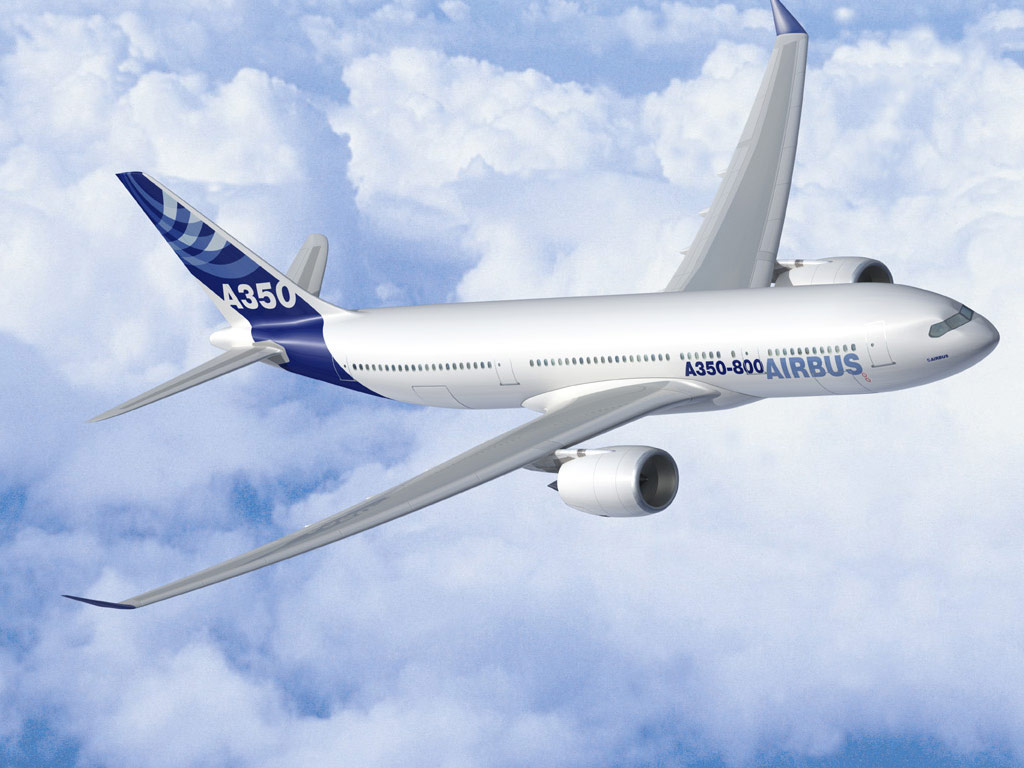
\includegraphics[height=50mm]{Figures/Airbus_A350.jpg}

% Title, author and degree
\vspace{1.0cm}
{\FontLb Intelligent Information System based on Android} \\ % <<<<< EDIT TITLE
%\vspace{0.2cm}
%{\FontMn Subtitle (optional)} \\
%\vspace{1.9cm}
\vspace{2.6cm}
{\FontMb Diogo Alexandre Ribeiro Ferreira} \\ % <<<<< EDIT NAME
\vspace{2.0cm}
%{\FontSn \coverThesis} \\
\vspace{0.3cm}
{\FontLb Introduction to Research in Electrical and Computer Engineering} \\ % <<<<< EDIT COURSE
\vspace{1.0cm}
{\FontSn %
\begin{tabular}{ll}
 \coverSupervisor: & Prof. Luís Miguel Teixeira D'Ávila Pinto da Silveira \\ % <<<<< EDIT NAME
                    %%& Dr. Full Name 2    % <<<<< EDIT NAME
\end{tabular} } \\
\vspace{1.0cm}
%{\FontMb \coverExaminationCommittee} \\
\vspace{0.3cm}
{\FontSn
\begin{tabular}{c}
%\coverChairperson:     Prof. Full Name          \\ % <<<<< EDIT NAME
%\coverSupervisor:      Prof. Full Name 1 (or 2) \\ % <<<<< EDIT NAME
%\coverMemberCommittee: Prof. Full Name 3           % <<<<< EDIT NAME
\end{tabular} } \\
\vspace{1.5cm}
{\FontMb January 2017} \\ % <<<<< EDIT DATE (corresponds to date of oral examination)
%
\end{center}

 % file "Thesis_FrontCover.tex"
%\cleardoublepage

%%%%%%%%%%%%%%%%%%%%%%%%%%%%%%%%%%%%%%%%%%%%%%%%%%%%%%%%%%%%%%%%%%%%%%%%%
%                                                                      %
%     File: Thesis_Dedication.tex                                      %
%     Tex Master: Thesis.tex                                           %
%                                                                      %
%     Author: Andre C. Marta                                           %
%     Last modified :  2 Jul 2015                                      %
%                                                                      %
%%%%%%%%%%%%%%%%%%%%%%%%%%%%%%%%%%%%%%%%%%%%%%%%%%%%%%%%%%%%%%%%%%%%%%%%

\null\vskip5cm%
\begin{flushright}
     Dedicated to someone special...
\end{flushright}
\vfill\newpage

 % file "Thesis_Dedication.tex"
%\cleardoublepage

%%%%%%%%%%%%%%%%%%%%%%%%%%%%%%%%%%%%%%%%%%%%%%%%%%%%%%%%%%%%%%%%%%%%%%%%%
%                                                                      %
%     File: Thesis_Acknowledgments.tex                                 %
%     Tex Master: Thesis.tex                                           %
%                                                                      %
%     Author: Andre C. Marta                                           %
%     Last modified :  2 Jul 2015                                      %
%                                                                      %
%%%%%%%%%%%%%%%%%%%%%%%%%%%%%%%%%%%%%%%%%%%%%%%%%%%%%%%%%%%%%%%%%%%%%%%%

\section*{\acknowledgments}

% Add entry in the table of contents as section
\addcontentsline{toc}{section}{\acknowledgments}

A few words about the university, financial support, research advisor, dissertation readers, faculty or other professors, lab mates, other friends and family...

 % file "Thesis_Acknowledgements.tex"
%\cleardoublepage

%%%%%%%%%%%%%%%%%%%%%%%%%%%%%%%%%%%%%%%%%%%%%%%%%%%%%%%%%%%%%%%%%%%%%%%%%
%                                                                      %
%     File: Thesis_Resumo.tex                                          %
%     Tex Master: Thesis.tex                                           %
%                                                                      %
%     Author: Andre C. Marta                                           %
%     Last modified :  2 Jul 2015                                      %
%                                                                      %
%%%%%%%%%%%%%%%%%%%%%%%%%%%%%%%%%%%%%%%%%%%%%%%%%%%%%%%%%%%%%%%%%%%%%%%%

\section*{Resumo}

% Add entry in the table of contents as section
\addcontentsline{toc}{section}{Resumo}

Inserir o resumo em Portugu\^{e}s aqui com o máximo de 250 palavras e acompanhado de 4 a 6 palavras-chave...

\vfill

\textbf{\Large Palavras-chave:} palavra-chave1, palavra-chave2,...

   % file "Thesis_Resumo.tex"
%\cleardoublepage

%%%%%%%%%%%%%%%%%%%%%%%%%%%%%%%%%%%%%%%%%%%%%%%%%%%%%%%%%%%%%%%%%%%%%%%%%
%                                                                      %
%     File: Thesis_Abstract.tex                                        %
%     Tex Master: Thesis.tex                                           %
%                                                                      %
%     Author: Andre C. Marta                                           %
%     Last modified :  2 Jul 2015                                      %
%                                                                      %
%%%%%%%%%%%%%%%%%%%%%%%%%%%%%%%%%%%%%%%%%%%%%%%%%%%%%%%%%%%%%%%%%%%%%%%%

\section*{Abstract}

% Add entry in the table of contents as section
\addcontentsline{toc}{section}{Abstract}

Insert your abstract here with a maximum of 250 words, followed by 4 to 6 keywords...

\vfill

\textbf{\Large Keywords:} keyword1, keyword2,...

 % file "Thesis_Abstract.tex"
%\cleardoublepage

% Table of contents
% Alterar para 2 ou apagar para deixar de aparecer 2.3.1.1
\setcounter{tocdepth}{3}
\setcounter{secnumdepth}{3}
\tableofcontents
%\cleardoublepage 

% List of tables
% Add entry in the table of contents as section
\phantomsection
\addcontentsline{toc}{section}{\listtablename}
% Generate list
\listoftables
%\cleardoublepage 

% List of figures
% Add entry in the table of contents as section
\phantomsection
\addcontentsline{toc}{section}{\listfigurename}
% Generate list
\listoffigures
%\cleardoublepage 

% Nomenclature
%
% entries of nomenclature list
%%%%%%%%%%%%%%%%%%%%%%%%%%%%%%%%%%%%%%%%%%%%%%%%%%%%%%%%%%%%%%%%%%%%%%%%%
%                                                                      %
%     File: Thesis_Nomenclature.tex                                    %
%     Tex Master: Thesis.tex                                           %
%                                                                      %
%     Author: Andre C. Marta                                           %
%     Last modified : 21 Jan 2011                                      %
%                                                                      %
%%%%%%%%%%%%%%%%%%%%%%%%%%%%%%%%%%%%%%%%%%%%%%%%%%%%%%%%%%%%%%%%%%%%%%%%
%
% The definitions can be placed anywhere in the document body
% and their order is sorted by <symbol> automatically when
% calling makeindex in the makefile
%
% The \glossary command has the following syntax:
%
% \glossary{entry}
%
% The \nomenclature command has the following syntax:
%
% \nomenclature[<prefix>]{<symbol>}{<description>}
%
% where <prefix> is used for fine tuning the sort order,
% <symbol> is the symbol to be described, and <description> is
% the actual description.

% ----------------------------------------------------------------------
% Roman symbols [r]
\nomenclature[ru]{$\bf u$}{Velocity vector.}
\nomenclature[ru]{$u,v,w$}{Velocity Cartesian components.}
\nomenclature[rp]{$p$}{Pressure.}
\nomenclature[rC]{$C_D$}{Coefficient of drag.}
\nomenclature[rC]{$C_L$}{Coefficient of lift.}
\nomenclature[rC]{$C_M$}{Coefficient of moment.}

% ----------------------------------------------------------------------
% Greek symbols [g]
\nomenclature[g]{$\rho$}{Density.}
\nomenclature[g]{$\alpha$}{Angle of attack.}
\nomenclature[g]{$\beta$}{Angle of side-slip.}
\nomenclature[g]{$\mu$}{Molecular viscosity coefficient.}
\nomenclature[g]{$\kappa$}{Thermal conductivity coefficient.}

% ----------------------------------------------------------------------
% Subscripts [s]
\nomenclature[s]{$x,y,z$}{Cartesian components.}
\nomenclature[s]{$i,j,k$}{Computational indexes.}
\nomenclature[s]{$\infty$}{Free-stream condition.}
\nomenclature[s]{ref}{Reference condition.}
\nomenclature[s]{$n$}{Normal component.}

% ----------------------------------------------------------------------
% Supercripts [t]
\nomenclature[t]{T}{Transpose.}
\nomenclature[t]{*}{Adjoint.}
\nomenclature[t]{GPS}{Global Positioning System.}
 % file "Thesis_Nomenclature.tex"
%
% Add entry in the table of contents as section
%\phantomsection
%\addcontentsline{toc}{section}{\nomname}
% Insert glossary/nomenclature section produced by MakeIndex
%\printnomenclature
%\cleardoublepage

% entries of glossary list
%%%%%%%%%%%%%%%%%%%%%%%%%%%%%%%%%%%%%%%%%%%%%%%%%%%%%%%%%%%%%%%%%%%%%%%%
%                                                                      %
%     File: Thesis_Glossary.tex                                        %
%     Tex Master: Thesis.tex                                           %
%                                                                      %
%     Author: Andre C. Marta                                           %
%     Last modified : 30 Oct 2012                                      %
%                                                                      %
%%%%%%%%%%%%%%%%%%%%%%%%%%%%%%%%%%%%%%%%%%%%%%%%%%%%%%%%%%%%%%%%%%%%%%%%
%
% The definitions can be placed anywhere in the document body
% and their order is sorted by <symbol> automatically when
% calling makeindex in the makefile
%
% The \glossary command has the following syntax:
%
% \glossary{entry}
%
% The \nomenclature command has the following syntax:
%
% \nomenclature[<prefix>]{<symbol>}{<description>}
%
% where <prefix> is used for fine tuning the sort order,
% <symbol> is the symbol to be described, and <description> is
% the actual description.

% ----------------------------------------------------------------------

%\glossary{name={\textbf{MDO}},description={Multi-Disciplinar Optimization is an engineering technique that uses optimization methods to solve design problems incorporating two or more disciplines.}}

%\glossary{name={\textbf{CFD}},description={Computational Fluid Dynamics is a branch of fluid mechanics that uses numerical methods and algorithms to solve problems that involve fluid flows.}}

%\glossary{name={\textbf{CSM}},description={Computational Structural Mechanics is a branch of structure mechanics that uses numerical methods and algorithms to perform the analysis of structures and its components.}}

%\newacronym{lvm}{LVM}{Logical Volume Manager}

\newacronym{gps}{GPS}{Global Positioning System}
\newacronym{wi-fi}{Wi-Fi}{Wireless Fidelity}
\newacronym{wlan}{WLAN}{Wireless Local Area Network}
\newacronym{ieee}{IEEE}{Institute of Electrical and Electronics Engineers}
\newacronym{ssid}{SSID}{Service Set Identifier} 
\newacronym{ios}{iOS}{iPhone Operating System}
\newacronym{rss}{RSS}{Received Signal Strength}
\newacronym{sig}{SIG}{Special Interest Group}
\newacronym{ble}{BLE}{Bluetooth Low Energy}
\newacronym{iot}{IoT}{Internet of Things} 
\newacronym{qrcodes}{QR Codes}{Quick Response Codes}
\newacronym{url}{URL}{Uniform Resource Locator}
\newacronym{nfc}{NFC}{Near-field Communication}
\newacronym{rfid}{RFID}{Radio-Frequency Identification} 
\newacronym{rssi}{RSSI}{Radio Signal Strength Indicator}
\newacronym{aoa}{AoA}{Angle of Arrival}
\newacronym{tof}{ToF}{Time of Flight}
\newacronym{rss}{RSS}{Received Signal Strength}
\newacronym{uuid}{UUID}{Universally Unique Identifier}
\newacronym{pdu}{PDU}{Protocol Data Unit}
\newacronym{url}{URL}{Uniform Resource Locator}
\newacronym{api}{API}{Application Programming Interface}
\newacronym{sdk}{SDK}{Software Development Kit}
\newacronym{uri}{URI}{Uniform Resource Identifier}
\newacronym{ceo}{CEO}{Chief Executive Officer}
\newacronym{ist}{IST}{Instituto Superior Técnico}
\newacronym{tx}{TX}{Transmission}
%\glsaddall % file "Thesis_Glossary.tex"

% Add entry in the table of contents as section
\phantomsection
\addcontentsline{toc}{section}{\glossaryname}
% Insert glossary section produced by MakeIndex
%\printglossary
%\cleardoublepage

%%%
\printglossary[type=\acronymtype]
%\printglossaries
\cleardoublepage

%%
% Set arabic numbering (1,2,...) after preface
%
\setcounter{page}{1}
\pagenumbering{arabic}

% ----------------------------------------------------------------------
%  Chapters
% ----------------------------------------------------------------------

\chapter{Introduction}
\label{chapter:introduction}

The \gls{iot} has been one of the major technology trends in the last years. \gls{iot} represents a general concept for the ability of network devices to sense and collect data from the world around us, and then share that data across the Internet where it can be processed and utilized for various interesting purposes. \gls{iot} is considered a revolution in terms of communication between devices.

The ability to determinate the position of devices or people inside buildings is one of the most important features in \gls{iot} and its development goes far beyond the red dot on a map, making positioning an important field of application for \gls{iot}. 
An application scenario, where the positioning data in stores leads to significant added value, is the anonymous tracking of customers itineraries. The system can analyse the data and conclude which products are more interesting or have greater popularity. It can also suggest other products associated to the ones seen before.

\gls{ble} is a key building block for the \gls{iot}, thanks to its pervasiveness due to the mobile devices support of Bluetooth 4.0, low-power consumption and protocol optimization for low-rate transmission.
Even though beacons are very simple, they are a technological advancement because they allow for indoor positioning and subsequently indoor behaviour tracking. They create a new seamless interaction that does not consume a lot of battery.

These \gls{ble} beacons are often described as "Smart Devices" in \gls{iot}. It is possible to extract information from certain objects just by bringing our device close to it. Non-processor entity whose data can be acquired and migrated over internet falls under these category. 

\begin{comment}

The system consists of base stations, mobile stations, a processing server and a web server. The base stations are implemented with custom software installed on WiFi and Bluetooth Low Energy (BLE) enabled Raspberry Pi’s. BLE beacons from Estimote are used as mobile stations. The base stations listen for mobile stations and the processing server collects information from the base stations. The web server hosts a custom web client developed in AngularJS that fetches real-time updates from the processing server and presents relevant information to first responders or system administrators. The processing server and web server may run on the same physical machine.
To estimate the position of a mobile station, RSSI based distance estimates are induced into a trilateration algorithm on the processing server. To increase the accuracy of the position estimates, a technique to continuously calibrate the path loss exponent was implemented.
------
Even though beacons are very simple, they are a technological advancement: They allow for indoor positioning (something that GPS is not able to provide) and subsequently indoor behavior tracking. They create a new seamless interaction that does not consume a lot of battery. Due to its simplicity, beacon technology does not need to battle as many standards as other IoT applications.
-------
Bluetooth Low Energy (BLE) is a key building block for the IoT, thanks to its pervasiveness (mobile devices support Bluetooth 4.0), low-power consumption and protocol optimization for low-rate transmission. 
BlueUp supports you in your projects based on BLE devices and beacons, offering state-of-art and enterprise-grade products and solutions, tailored for your needs.
\end{comment}

\begin{comment}
-------
3.2 What are Smart Objects?

We find the mention of "Smart Objects" and "Smart Devices" quite often in general defination and description of IoT alongside network connectivity of embedded system. But what exactly are smart object?

Quote:
A Smart Object is an object that can describe its own possible interactions. 

Any object which not only has a state, which has certain data associated with a state but an object which can also determine nature of connectivity, duration of connectivity and connectivity protocol are called smart objects.

Radio Frequency Identification (RFID), Bluetooth Low Energy (BLE), and Near Field Communication (NFC)  makes it possible to use our phone as readers. We can extract information from certain objects just by tapping it or bringing our device close to it. RFID tags does not have any embedded system nor does a NFC tag has. But data can still be brought to internet by reading through a reader. These are called smart objects.  Non-processor entity whose data can be acquired and migrated over internet falls under these category. 
\end{comment}

%url{http://www.pcworld.com/article/2000276/a-brief-history-of-gps.html}

%\url{http://info.atollic.com/hs-fs/hub/460400/file-2653641781-jpg/Blog/iot.jpg}

%\url{https://www.infsoft.com/blog-en/articleid/135/internet-of-things-and-indoor-positioning#}
\section{Problem definition}
\label{section:problem}

Commercial, ludic and scientific spaces, most of the times, cannot or have difficulty in directing users to their interest. Spaces use different ways to achieve this goal, for example, stores use discounts to increase their sales of certain products. The fact that sometimes discounts go unnoticed is related to the way owners or administrators spread the information, which does not guarantee reaching efficiently the customers. It would be easier, if the customers could receive the information in a mobile phone application, at the right time and in the right situation. On the other hand, the administrators have doubts where to put the information available to the users. It would be useful, if the information about the localization of their consumers was provided to the owners or administrators. 
Therefore, arises the need for a positioning system in an indoor environment that can localize devices and transmit the information that both clients and owners want.
%
%acho que o problema não é o receberem ou não toda a informação e receberem-na no telefone ou de outra forma.  O problema é receberem-na no momento e situação certo.  É para isso que o conhecimento da posição de um cliente dentro de uma loja ajuda.  O telefone é um mero instrumento que é pratico usar pois toda a gente tem um (assume-se).
%%%%%%%%%%%%%%%%%%%%%%%%%%%%%%%%%%%%%%%%%%%%%%%%%%%%%%%%%%%%%%%%%%%%%%%%
\section{Motivation}
\label{section:motivation}
Having in mind the need for a positioning system in an indoor environment, many different solutions for achieving the user's positioning have been proposed. An interesting setting is one where Bluetooth beacons can interact with mobile phones and a processing server. The mobile phone has the hardware necessary for \gls{wi-fi} and \gls{ble} enabled. The mobile phone application listens for \gls{ble} beacons advertisements and the processing server collects information from the mobile phone. In Figure \ref{fig:motiv} a visual description of this system is given.
To estimate the position of a mobile phone, \gls{rssi} based distance estimates are induced into an algorithm on the processing server, it is possible to do this calculation in the mobile phone application if the mobile phone has sufficient capacity to do this calculus.

\begin{figure}[!htb]
	\centering
	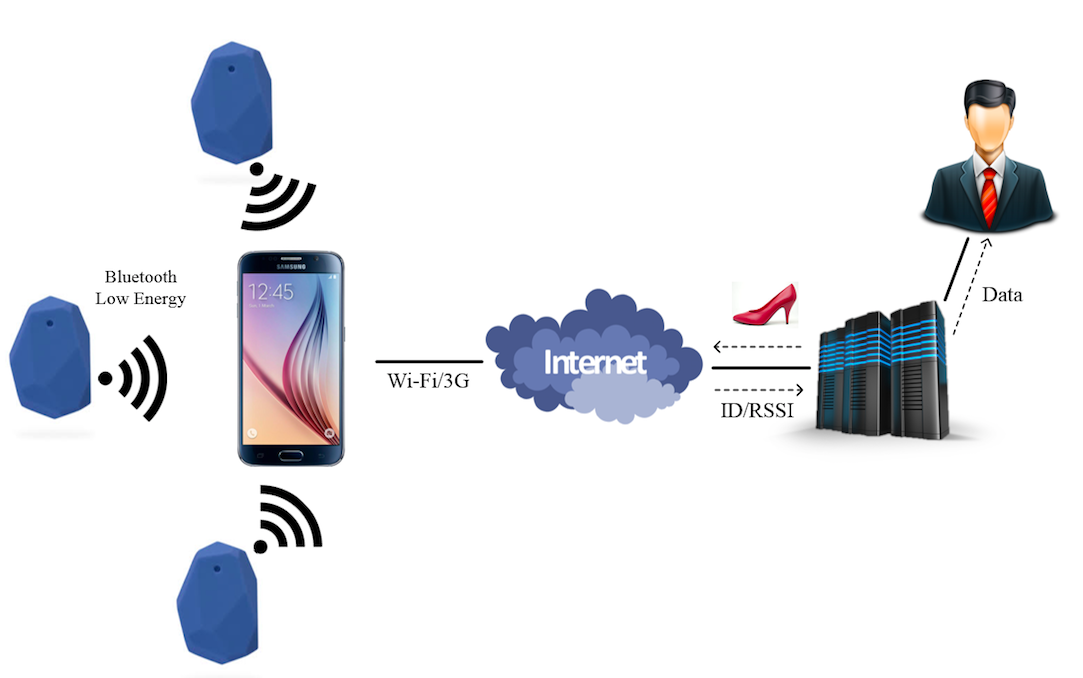
\includegraphics[width=1\textwidth]{Figures/architecture.png}
	\caption[Architecture of the positioning system]{Architecture of the positioning system.}
	\label{fig:motiv}
\end{figure} 

\begin{comment}

The idea of having access control be aware of a user’s location is an interesting concept and an ongoing research area. Many different solutions for achieving this location awareness have been proposed, for instance WiFi signal strength triangulation, radio- and ul- trasound transmitters, combinations of WiFi signals and accelerometers, etc. Issues with existing solutions include overspecialization, custom hardware requirements or active user interaction. A new method for achieving Location Aware Access Control (LAAC) should thus be simple, affordable, require no actual end-user interaction to function, and support as many modern portable devices as possible. 

A simple-to-use and reliable solution will hopefully lead to more security systems making use of location data, all while accruing relatively small costs. This is where the idea of BLE beacons comes in. Many modern portable devices supports receiving and transmitting BLE signals and the transmitters are cheap, small and energy efficient.

------------
"50 billion connected devices by 2020". Ericsson’s former \gls{ceo}, Hans Vestburg, stated it in a 2010 presentation to shareholders\footnote{https://www.ericsson.com/thecompany/press/releases/2010/04/1403231}. The next year, Dave Evans, who worked for Cisco\footnote{http://www.cisco.com}, published the same prediction in~\citep{cisco}. With this in mind, new technologies have been developed and improved to facilitate the communication between devices. Therefore, a revolution has arisen in the way positioning systems have been deployed.
\end{comment}

%http://www.ics.uci.edu/~cs237/ProjectSlidesSpring2015/15.pdf

%http://academia.stackexchange.com/questions/44784/how-to-explain-things-in-the-motivation-section-of-a-mathematical-paper-without

%\url{http://www.fiercewireless.com/wireless/ericsson-backs-away-from-expectation-50b-connected-devices-by-2020-now-sees-26b}

%\url{http://spectrum.ieee.org/tech-talk/telecom/internet/popular-internet-of-things-forecast-of-50-billion-devices-by-2020-is-outdated}
%%%%%%%%%%%%%%%%%%%%%%%%%%%%%%%%%%%%%%%%%%%%%%%%%%%%%%%%%%%%%%%%%%%%%%%%

%%%%%%%%%%%%%%%%%%%%%%%%%%%%%%%%%%%%%%%%%%%%%%%%%%%%%%%%%%%%%%%%%%%%%%%%
\section{Objectives}
\label{section:objectives}

The objective of this work consists in the elaboration of a system in an indoor environment that uses positioning methods to determine the position of users in a certain space.
A mobile phone application must be developed. This application receives location information from a set of beacons placed in an indoor environment. Based on that, it gets relevant information from a local or remote database and makes that information available to the user dynamically, as the user moves and his or hers position changes.
The accuracy of positioning obtained with \gls{ble} technology and the positioning methods is also checked.

%Isto continua telegrafico.  Nunca falas da aplicação?  Não é objectivo do trabalho também?  Que tal dizeres que o sistema consistirá numa aplicação que recebe informação de localização de um conjunto de beacons colocados num indoor environment e que com base nessa localização obtem informação relevante duma base de dados local (ou remota) e disponibiliza essa informação dinamicamente ao utilizador à medida que ele se desloca e a sua posição se altera???

%%%%%%%%%%%%%%%%%%%%%%%%%%%%%%%%%%%%%%%%%%%%%%%%%%%%%%%%%%%%%%%%%%%%%%%%
\section{Document Outline}
\label{section:outline}

This document is organized as follows:

\textbf{Chapter 2 (Background)}
provides the necessary background information and the state of the art related work;

\textbf{Chapter 3 (Design Choices)}
introduces the architecture of the positioning system, describes its components and implementation scenarios;

\textbf{Chapter 4 (Thesis Planning)}
presents a Gantt diagram and an explanation about the planning of the work that is going to be done next semester.
 % file "Thesis_Introduction.tex"
%\cleardoublepage

\chapter{Background}
\label{chapter:background}

%Positioning has been around since the need to locate warships arose. 
Technology has evolved and due to that, with the use of positioning methods, nowadays it is used to locate people and devices indoors. 

This chapter discusses about the knowledge needed prior to the implementation of an indoor positioning system. Section~\ref{section:Technologies} introduces the technologies used to calculate the position and achieve the positioning system referred in~\ref{section:objectives}, such as: \gls{gps}, \gls{wi-fi}, Bluetooth, \gls{qrcodes}, \gls{nfc} and \gls{rfid}.
In~\ref{section:methods}, several methods about positioning, for example Lateration and Fingerprinting, are introduced and then in~\ref{section:protocols} the latest beacons, its characteristics and limitations in indoor environments are going to be introduced. ~\ref{section:manufacturers} makes reference to the different types of beacons manufacturers on the market. In ~\ref{section:aplications} are commented the functionalities of the applications already existing in the market. The Section~\ref{section:summarybackground} does a summary about everything that was mentioned before.

%%%%%%%%%%%%%%%%%%%%%%%%%%%%%%%%%%%%%%%%%%%%%%%%%%%%%%%%%%%%%%%%%%%%%%%%

\section{Technologies}
\label{section:Technologies}
Mobile devices must be able to calculate their position, using a specific technology, in order to be used in a positioning system. Several types of technologies can obtain the position of a device in an indoor environment.
The most well-known technologies for positioning are introduced below with the corresponding advantages and limitations for its use in indoor systems.

\subsection{GPS}
\label{subsection:gps}

\gls{gps}\footnote{http://www.gps.gov} is a satellite system that is used to provide geolocation and time information to a \gls{gps} receiver anywhere on Earth.
In order to work correctly, in other words, without signal weakens or distortions making the result inaccurate, \gls{gps} receivers need to have a line of sight to four or more \gls{gps} satellites.

\gls{gps} uses trilateration as the technique to get the position of the receiver. With a view to calculate the position, the receiver needs the location of the satellites and the distance from the receiver to each one of those satellites. \gls{gps} receiver measures the distance to a \gls{gps} satellite using the travel time of radio signals.

The current \gls{gps} consists of three segments: the space segment, the control segment and the user segment.
The user segment is the part of the \gls{gps} system the user is most aware of. It is often simply equated with a \gls{gps} receiver, which is, only a part of the user segment. Its configuration actually depends on the application it is used for~\citep{KupperAxel}.
\gls{gps} is one of the most successful and popular positioning systems in outdoor environments. 

Despite being popular, it is not appropriate to indoor environments because microwaves will be attenuated and scattered by roofs, walls and other objects making it unsuitable for indoor positioning estimation due to its low accuracy. 

%An example of the malfunction in the use of \gls{gps} in indoor location applications, is one of the most downloaded applications in App Store history: Pokémon Go\footnote{http://www.pokemongo.com}. While playing the game indoor, a warning would appear saying that the user would be driving without even moving - this event is called \gls{gps} drift.

Another limitation of \gls{gps}, is the fact that it cannot detect altitude, being impossible to distinguish different floors.

Therefore, some studies were made in order to improve indoor positioning with \gls{gps}, using \gls{gps} repeaters. However, the cost of installing these repeaters was high and the accuracy did not improve as much as expected~\citep{GPStransmitters}.

%%%%%%%%%%%%%%%%%%%%%%%%%%%%%%%%%%%%%%%%%%%%%%%%%%%%%%%%%%%%%%%%%%%%%%%%
\subsection{Wi-Fi}
\label{subsection:wifi}
\gls{wi-fi}\footnote{http://www.wi-fi.org} is a technology that enables devices to connect to a \gls{wlan} using radio waves.

It is based on the \gls{ieee} 802.11 standard.
\gls{wi-fi} compatible devices connect to the Internet via a wireless access point which does the access to a \gls{wlan} network. 

This technology is widely used all over the world and is one of the most common local area networking techniques today.

However, its use to indoor positioning brings several problems to the users, such as:

\begin{itemize}
\item Limitation of the update rate due to the increased duration of passive \gls{wi-fi} scans- where the device waits for a \gls{ssid};

\item Reducing \gls{wi-fi} throughput, increasing network traffic as well as reducing privacy due to the use of frequent active Wi-Fi scans, where the device to be positioned broadcasts a query;

\item \gls{wi-fi} does not require the signal strength value to be reported in any specific unit, which several positioning methods depend on. Because of this, some mobile platforms have not allowed the access to the \gls{wi-fi} scan data. For instance, Apple’s \gls{ios} only allows \gls{rss} readings from the connected access point~\citep{fingerprintingble}, making it impossible to use more advanced positioning methods to calculate the position.
\end{itemize}

\subsection{Bluetooth}
\label{subsection:bluetooth}
Bluetooth\footnote{https://www.bluetooth.com} is a wireless standard technology that connects devices, fixed or mobile, together over short distances and is becoming more and more popular in modern technologies. It can be found in all sorts of devices and areas of consumer goods from mobile phones, headsets, tablets, etc. 

Bluetooth technology was created as an open standard to allow connectivity between different products leading to a cooperation between industries.

The Bluetooth \gls{sig} manages the development of Bluetooth standards and the licensing of the Bluetooth Technologies. Since Bluetooth technology is built upon a core specification and layered with different services, the \gls{sig} has worked to ensure its interoperability. 

In order to achieve better values of power consumption, Bluetooth suffered an update to Bluetooth 4.0 where it included \gls{ble}, gaining a lot of attention in the Internet of Things concept.

\gls{ble} is the power consumption and application friendly version of Bluetooth built for the \gls{iot}. \gls{ble} has a standard wireless protocol that allows for multi-vendor interoperability and has several power consuption modes, such as: ultra-low peak, average and idle mode that gives the ability to run for several months on a standard coin-cell battery.

\gls{ble} communication works in two different modes: advertising and connection.
Advertising is a one-way discovery mechanism. Devices which want to be discovered transmit packets of data repeatedly in intervals of time. The shorter the interval, the shorter the battery life is going to be and the faster the device can be discovered.
\gls{ble} devices can operate in advertisement mode only, in which all the information is contained in the advertisement.

\subsection{QR Codes}
\label{subsection:qrcodes}
\gls{qrcodes} are a two-dimension bade code which can be read by an application downloaded on a mobile device, that uses the camera to collect and then decode the data from the image. 

\gls{qrcodes} can be used to link the user directly to a \gls{url}, send a text message, call a phone number, decode a secret message or download contact information. QR codes can be freely generated in the Internet.

To read a small size QR code, for example a QR code in a magazine, the device should be at a maximum distance of 10 centimetres. \gls{qrcodes} can also be read from further away but their size should increase, for example, \gls{qrcodes} on sign posts or buildings must be scanned in a distance between 3 and 8 meters.

However, one limitation of this technology is the fact that it requires user interaction, that means the user needs to be aware of this codes to collect them.

\subsection{NFC}
\label{subsection:nfc}
\gls{nfc}\footnote{http://nearfieldcommunication.org} is a contactless form of communication between devices because it allows the user to send information over a \gls{nfc} compatible device, without needing to place the devices together or through several steps to make a connection. 

\gls{nfc} transmissions can occur in two modes: active and passive.
In the active mode, both devices generate the radio signal.
In Passive, only one device generates the radio signal of the connection and the second is powered by this. This mode can be used on items that do not need to receive direct power.

As in \gls{qrcodes}, to use \gls{nfc} the user needs to be aware of this devices because \gls{nfc} has a very short range, up to 4 or 5 centimetres. The need for a reader is another limitation of this type of technology.


\subsection{RFID}
\label{subsection:rfid}
\gls{rfid} is a technology that uses radio frequency signals to capture data. The method of identification in \gls{rfid} consists in storing a serial number that identifies an object or a person, on a microchip.

An \gls{rfid} system has several basic components, including \gls{rfid} readers, \gls{rfid} tags and the communication between them.

The read range of \gls{rfid} tags vary, some tags can be read from 30 meters and others only from 10 centimetres. 

\gls{rfid} tags can be categorized, as \gls{nfc}, in two categories: active or passive, depending if they operate with or without battery.

\subsection{Comparison}
\label{subsection:comparisontechnologies}

After introducing these technologies, it is possible to make a comparison between them, with the objective of exposing their differences to help in further technology selection in terms of cost, accuracy, precision, complexity, scalability and robustness. \gls{nfc} and \gls{qrcodes} present the same characteristics as \gls{rfid} which was the chosen technology from the three to be compared with the others.
This comparison can be seen in Table~\ref{tab:technodif}~\citep{SurveyofWireless}.

%%%%%%%%%%%%%%%%%%%%%%%%%%%%%
\begin{table}[!htb]
  \renewcommand{\arraystretch}{2} % more space between rows
  \centering
  \resizebox*{\textwidth}{!}{
  \begin{tabular}{lccccc p{1.5cm}}
    \toprule
   \textbf{Technologies} &Accuracy&Precision&Scale&Complexity&Robustness&Cost\\
    \midrule
    \textbf{GPS}   		&5m-50m&50\% within 25m&Good&High&Poor&Medium \\
    \textbf{Wi-Fi}		&3~5m&50\% within 2.5m and 90\% within around 5.9m&Good&Moderate&Good&Low\\
    \textbf{Bluetooth}	&2m&95\% within 1m&Nodes placed every 2-15m&positioning delay 15-30s&Poor&Medium\\
    \textbf{RFID}		&$<$2m&50\% within 1m&Nodes placed densely&Medium&Poor&Low\\
    \bottomrule
  \end{tabular}
  }
  \caption[Technologies' Differences]{Technologies' Differences.}
  \label{tab:technodif}
\end{table}

%%%%%%%%%%%%%%%%%%%%%%%%%%%%%%%%%%%5
\section{Positioning Methods}
\label{section:methods}
Several methods can be used to estimate the position of devices. The estimation can use one or more methods. In this section the necessary measures and methods for the realization of the estimation are approached.
A lot of measurements can be used to calculate the position of a device, such as \gls{aoa}, \gls{tof} and \gls{rss}, Received Signal Strength. However, mobile devices do not support the hardware necessary to obtain some types of measurements, for instance, the \gls{aoa} of the received signal. In indoor systems, due to its short distance, it is not appropriate to use the \gls{tof} of a signal because the time difference between sending and receiving is very small. 
\gls{rss} is an effective measure to the calculation of a position in an indoor system and it can be collected in mobile devices.


\subsection{Received Signal Strength}
\label{subsection:receivedsignal}
\gls{rss} can be used to calculate the distance, calculating the path loss when the signal travels from the sender to the receiver. The simplest model is the Friis free space model equation, which allows the consideration of environmental parameters only in the form of the path-loss gradient. \gls{rssi} can be calculated with the equation in~\ref{eq:rssi}.
\begin{equation}
\label{eq:rssi}
RSSI = -(10\cdot n)\log_{10}(d) +A
\end{equation}

\gls{rssi} in $dBm$, $n$ is the signal propagation constant, $d$ is the distance between the sender and the receiver and $A$ is the reference received signal strength in $dbm$ for the distance of one meter.
Equation~\ref{eq:distance} used to calculate the distance can be derived from~\ref{eq:rssi}.

\begin{equation}
\label{eq:distance}
d =10^{\frac{RSSI-A}{-10\cdot n}}
\end{equation}

In indoor environments, due to the short distances, can be really hard to measure the travelling time from the sender to the receiver, so the most used methods use \gls{rssi} values.

The methods of positioning to locate devices can be divided into two groups: active and passive~\citep{surveylocation}. 
Active positioning techniques determine the position of a device based on signals received.
Passive positioning techniques determine the position based on the information that the main sensor receives indirectly  from the environment. 


\subsection{Proximity Sensing}
\label{subsection:proximity}
Proximity Sensing is an active positioning technique and is the easiest and most widespread method to obtain the position of a target. It relies on the limited range of radio, infrared or ultrasound signals coverage.

In indoor systems, proximity sensing has been implemented in various research projects, since its accuracy works better for this kind of systems. The position of the terminal is determined from the position of the access point from which the terminal receives a greater \gls{rss} signal.

\subsection{Lateration}
\label{subsection:lateration}
Lateration is an active process of estimating the position of the target by measuring the distances to a set of points with a known location. The position is estimated using geometric figures such as circles, triangles or spheres. In order for the position to be estimated, at least three different base stations are needed. When the number of base stations used is three, lateration is also known as trilateration showed in Figure~\ref{fig:trilaterationimag}.

Suppose there are three distinct reference nodes  $p_{i}=
\left ( x_{i},y_{i} \right ),i =1,2,3$ in a two dimensional space and the coordinate 
$\left ( x_{0},y_{0} \right ) $ of an unknown node $p$ is going to be calculated, using $r_{i},i =1,2,3$.

\begin{figure}[!htb]
  \centering
  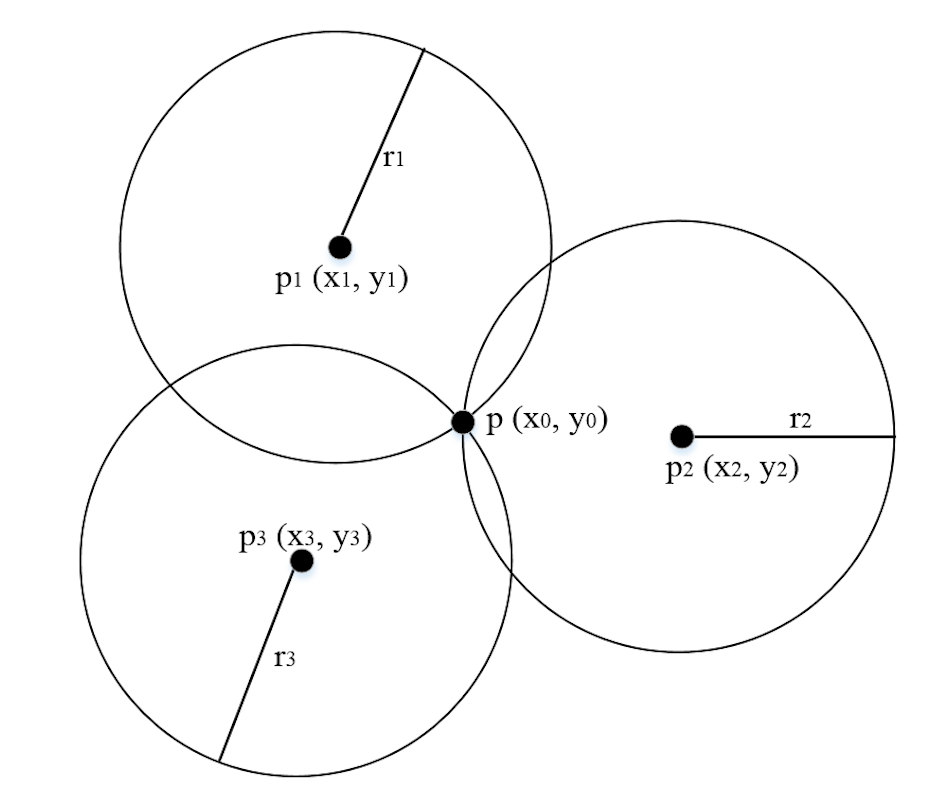
\includegraphics[width=0.5\textwidth]{Figures/trilat.png}
  \caption[Trilateration]{Trilateration}
  \label{fig:trilaterationimag}
\end{figure}

The following system of equations based on trilateration method is obtained:
\begin{equation}
\begin{cases} 
\left (x_{0}-x_{1}\right )^{2}+
\left (  y_{0}-y_{1}\right )^{2}={r_{1}}^{2}\\
\left (x_{0}-x_{2}\right )^{2}+\left (  y_{0}-y_{2}\right )^{2}={r_{2}}^{2}\\
\left (x_{0}-x_{3}\right )^{2}+\left (  y_{0}-y_{3}\right )^{2}={r_{3}}^{2}
\end{cases}
\end{equation}
From the previous system of equations the position of the unknown node $p$ is derived:
\begin{equation}
\begin{cases} 
x_{0} =\frac{1}{\Delta}\left ( 2T_{1}\left ( y_{1}-y_{3} \right )-2T_{2}\left ( y_{1}-y_{2} \right ) \right )
\\y_{0} =\frac{1}{\Delta}\left ( 2T_{2}\left ( x_{1}-x_{2} \right )-2T_{1}\left ( x_{1}-x_{3} \right ) \right )
\end{cases}
\end{equation}
where $ T_{1} = {r_{2}}^{2}-{r_{1}}^{2}-{x_{2}}^{2}+{x_{1}}^{2}-{y_{2}}^{2}+{y_{1}}^{2}
, T_{2} = {r_{3}}^{2}-{r_{1}}^{2}-{x_{3}}^{2}+{x_{1}}^{2}-{y_{3}}^{2}+{y_{1}}^{2}
$ and 
$\Delta  = 4\left ( \left ( x_{1}-x_{2} \right ) \left ( y_{1}-y_{3} \right )-\left ( x_{1}-x_{3} \right )\left ( y_{1}-y_{2} \right )\right )$.

The position of the target can only be estimated if the three nodes are not in a straight line. Moreover, the nodes should not be close to each other, otherwise $\Delta$ will become too small to estimate the unknown node~\citep{novelref}.

\subsection{Angulation}
\label{subsection:angulation}
Angulation is an active process of estimating the position of the target by using the angles between known base stations and the mobile device. To estimate the position, at least two base stations are needed. However, it is required that either base stations or terminals are equipped with antenna arrays. Suppose two distinct reference nodes exist $p_{i}=\left ( x_{i},y_{i} \right ),i =1,2$ using the angles $\alpha_{i}, i=1,2$ it is possible to estimate the position of the an unknown node $p$ as depicted in Figure~\ref{fig:angulation}~\citep{KupperAxel}.
\begin{figure}[!htb]
  \centering
  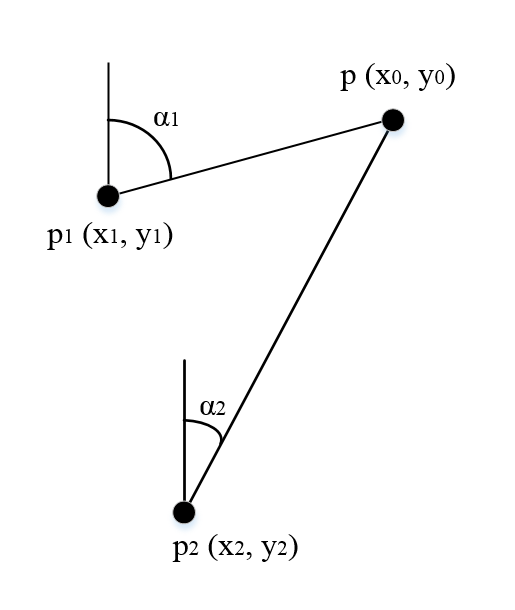
\includegraphics[width=0.3\textwidth]{Figures/ang.png}
  \caption[Angulation]{Angulation.}
  \label{fig:angulation}
\end{figure}

\subsection{Fingerprinting}
\label{subsection:fingerprinting}
Fingerprinting is a passive localization method and can be divided in two phases.

In the first phase, it is necessary to collect the \gls{rssi}, Radio Signal Strength Indicator, data along the locations where the user is expected to be, in order to construct a map of \gls{rssi} values, making this method environment related. These values are then stored in the fingerprinting database so that they can be used later. 
 
In the second phase, the device collects the \gls{rssi} values and compares them with the values in the fingerprinting database, to identify the values which relate the most to those obtained. Several methods of comparison can be used, such as: probabilistic methods, k-Nearest Neighbours, neutral networks, support vector machine and smallest M-vertex polygon~\citep{ImprIndoorLocal}.

	
\section{Beacons Protocols}
\label{section:protocols}
Beacons are small devices which only use the advertisement mode in \gls{ble}. They transmit packets of data in regular intervals of time, which can be then received by other devices like smartphones. The emitted message contains information that the receiving device can use to identify the beacon and to compute its relative distance to the beacon. The receiving device may use this information as a contextual trigger to execute procedures and implement behaviours that are relevant to being in proximity to the transmitting beacon.

There are several beacon protocols that define a message format for beacon advertisements, such as: 
\begin{itemize}
\item iBeacon,
\item AltBeacon,
\item Eddystone,
\item URIbeacon.
\end{itemize}

\subsection{iBeacon}
\label{subsection:ibeacon}
iBeacon\footnote{https://developer.apple.com/ibeacon/} is a protocol developed by Apple and was the first beacon protocol in the market. iBeacon works with Apple's \gls{ios} and Google's Android. It is widely supported, simple and easy to implement and has a reliable performance on \gls{ios}.
iBeacon broadcast segments of data, displayed in Figure~\ref{fig:ibeaconadv}, such as:
\begin{itemize}
\item iBeacon Prefix, containing the hexadecimal data: 0x0201061AFF004C0215.
\item \gls{uuid}, that identifies the beacon.
\item Major number, that identifies a subset of beacons within a large group.
\item Minor number, that identifies a specific beacon.
\item \gls{tx} power level in 2's complement, indicating the signal strength one meter from the device. This number must be calibrated for each device by the user or manufacturer. \gls{tx} power field is used with the measured signal strength to determine how far away the beacon is from the smart phone~\citep{smartanaibeacon}.
\end{itemize}

\begin{figure}[!htb]
  \centering
  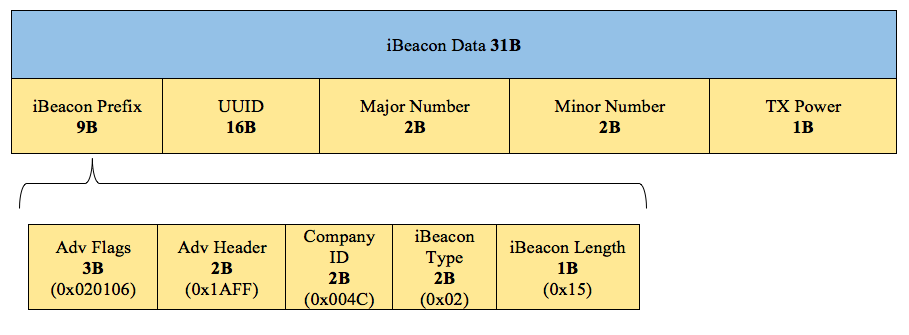
\includegraphics[width=1\textwidth]{Figures/ibeacon_v2.png}
  \caption[iBeacon Advertisement Format]{iBeacon Advertisement Format.}
  \label{fig:ibeaconadv}
\end{figure}

\subsection{AltBeacon}
\label{subsection:altbeacon}
AltBeacon\footnote{http://altbeacon.org} is a protocol specification provided by Radius Networks that defines a message format for proximity beacon advertisements. 
The AltBeacon advertisement makes use of the Manufacturer Specific Advertising Data structure as defined in Bluetooth 4.0, Volume 6, Part B, Section 2.3 Advertising Channel \gls{pdu}~\citep{roleofble_altbeacon}.
The AltBeacon advertisement, shown in Figure~\ref{fig:altbeaconadv}, is made up of:
\begin{itemize}
\item 1-byte length field;
\item 1-byte type field;
\item 2-byte company identifier, as prescribed by the Manufacturer Specific Advertising Data structure format;
\item 24 bytes containing the beacon advertisement data.
\end{itemize}

\begin{figure}[!htb]
  \centering
  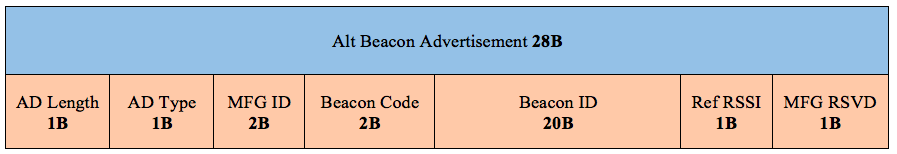
\includegraphics[width=1\textwidth]{Figures/altbeacon_v2.png}
  \caption[AltBeacon Advertisement Format]{AltBeacon Advertisement Format.}
  \label{fig:altbeaconadv}
\end{figure}

\subsection{Eddystone}
\label{subsection:eddystone}
Eddystone\footnote{https://github.com/google/eddystone} is an open beacon protocol developed by Google and designed with transparency. It can be detected by both Android and \gls{ios} devices. Eddystone protocol builds on lessons learned from working with industry partners in existing deployments, as well as the wider beacon community. Eddystone can have different types of payloads in the frame format, shown in Figure~\ref{fig:eddystoneadv}, such as:
\begin{itemize}
\item Eddystone-UID: A unique, opaque ID with a 10-byte Namespace component and a 6-byte Instance component. 
\item Eddystone-URL: A compressed \gls{url} that, once parsed and decompressed, is directly usable by the client. 
\item Eddystone-TLM: Beacon status data that is useful for beacon fleet maintenance, and powers Google Proximity Beacon \gls{api}'s diagnostics endpoint. -TLM should be interleaved with an identifying frame such as Eddystone-UID or Eddystone-EID (for which the encrypted eTLM version preserves security). 
\item Eddystone-EID: A time-varying beacon frame that can be resolved to a stable identifier by a linked resolver, such as Proximity Beacon \gls{api}~\citep{campus_survey}. 
\end{itemize}

\begin{figure}[!htb]
  \centering
  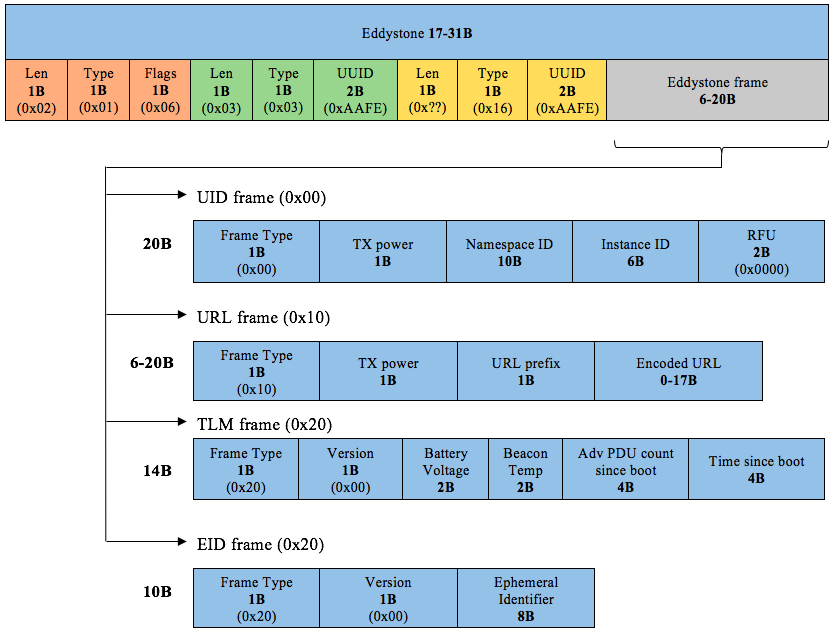
\includegraphics[width=1\textwidth]{Figures/eddystone_v3.png}
  \caption[Eddystone Advertisement Format]{Eddystone Advertisement Format.}
  \label{fig:eddystoneadv}
\end{figure}

\subsection{URIbeacon}
\label{subsection:uribeacon}
URIBeacon\footnote{https://github.com/google/uribeacon} is an open beacon protocol developed by Google and is part of Google’s project Physical Web initiative. URI beacon uses the payload to give short links to the internet via \gls{ble} advertising packets. The beacons using this protocol are meant to be updated with new information over time. Since they provide a link to the internet, they do not need a database to give meaning to the information they send. The URIBeacon advertisement format is displayed in the Figure~\ref{fig:uribeaconadv}.

\begin{itemize}
\item 19 bytes are used to encode the \gls{uri}.
\item The prefix and the suffix are encoded in two bytes. However, limiting the number of bytes only allows certain domains to be encoded. URIbeacons are supposed to be used with \gls{url} shortening services like goo.gl, bit.ly, tin.ly which will shorten any long \gls{url} to eight to ten bytes.
\end{itemize}
 

\begin{figure}[!htb]
  \centering
  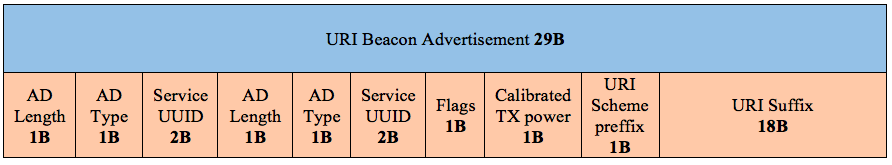
\includegraphics[width=1\textwidth]{Figures/uribeacon_v2.png}
  \caption[URIbeacon Advertisement Format]{URIbeacon Advertisement Format.}
  \label{fig:uribeaconadv}
\end{figure}

\subsection{Comparison}
\label{subsection:comparison}

After introducing these protocols, it is important to identify the biggest differences between them, which allows to choose between the protocol that makes the most sense to use in a project. These differences are summarized in the Table~\ref{tab:protocolsdif}.

\begin{table}[!htb]
  \renewcommand{\arraystretch}{2} % more space between rows
  \centering
  \resizebox*{\textwidth}{!}{
  \begin{tabular}{lcccc p{1.5cm}}
    \toprule
   \textbf{ Protocols      } &iBeacon&Eddystone&AltBeacon&URIBeacon\\
    \midrule
    \textbf{Developed by}    &Apple&Google&Radius Networks&Google\\
    \textbf{Open }			&No&Yes&Yes&Yes\\
    \textbf{Compatibility}	&\begin{tabular}[t]{@{}c@{}}Android and iOS,\\ but native only for iOS.\end{tabular}&Android and iOS.&Android and iOS.& Android and iOS.\\
    \textbf{\begin{tabular}[t]{@{}c@{}}Types of data \\broadcasted\end{tabular}}  & Unique ID number.&\begin{tabular}[t]{@{}c@{}}Unique ID number, or a URL \\address or sensor telemetry.\end{tabular}& Unique ID number.&Uniform Resource Identifier (URI).\\
    \textbf{API	}	&None&\begin{tabular}[t]{@{}c@{}}Nearby API, Proximity Beacon\\API and  Places API\end{tabular}&Android Library API&Same as Eddystone\\
    \bottomrule
  \end{tabular}
  }
  \caption[Beacons Protocols.]{Beacons Protocols.}
  \label{tab:protocolsdif}
\end{table}

The protocols can be divided in two groups where an ID number or an \gls{url} is broadcasted. iBeacon and AltBeacon are integrated in the group where an ID number is broadcasted and URIBeacon is integrated in the group where an \gls{url} is broadcasted. Eddystone can integrate both groups.

These two groups work in different ways:
\paragraph{ID number broadcasted}
\label{paragraph:sidnumber}
A scanning application reads the ID number and compares it with a database to get information about the beacon.
The beacon itself carries no descriptive information - it requires external database to be used. 

\paragraph{URL broadcasted} 
\label{paragraph:urlbroadcasted}
A scanning application reads the \gls{url} and opens it in a browser, it does not need a database to get the information.
The beacon information that is broadcasted in this case needs to be updated regularly.

\section{Manufacturers}
\label{section:manufacturers}
There is a wide variety of beacon manufacturers on the market. To choose the most appropriate beacon some criteria must be followed:
\begin{itemize}
\item Battery life and its rechargeability; 

\item Transmission rate and power.

\end{itemize}
The most common beacon manufacturers in the market are: Estimote, Gimbal, Bluvision and Kontakt.io~\citep{Statler}. Despite the existence of these well-known manufactures, other manufacturers exist, for example: Quuppa, BlueCats, BlueSense, Gelo, Glimworm, Sensorberg, Sonic Notify, Sensoro, Zebra, etc. There are still some electronics companies that provide low cost beacons such as: Shenzhen Sky Electronics Manufactory and Iotton. In this section, some of these manufacturers and their products are introduced and compared.

\subsection{Estimote} 
\label{subsection:estimote}
Estimote\footnote{http://estimote.com} is a technological start-up that sells beacons and has the largest developer community on the beacon system using its \gls{sdk}. Estimote is well known for the appealing image of the products and its packaging. Estimote recommends to application developers, when they are making simple proximity applications, to start with their Proximity Beacons, presented in Figure~\ref{fig:estimotebeacon}. Their beacons support both iBeacon and Eddystone, being capable of broadcasting both URL or ID Number. 

\begin{figure}[!htb]
  \centering
  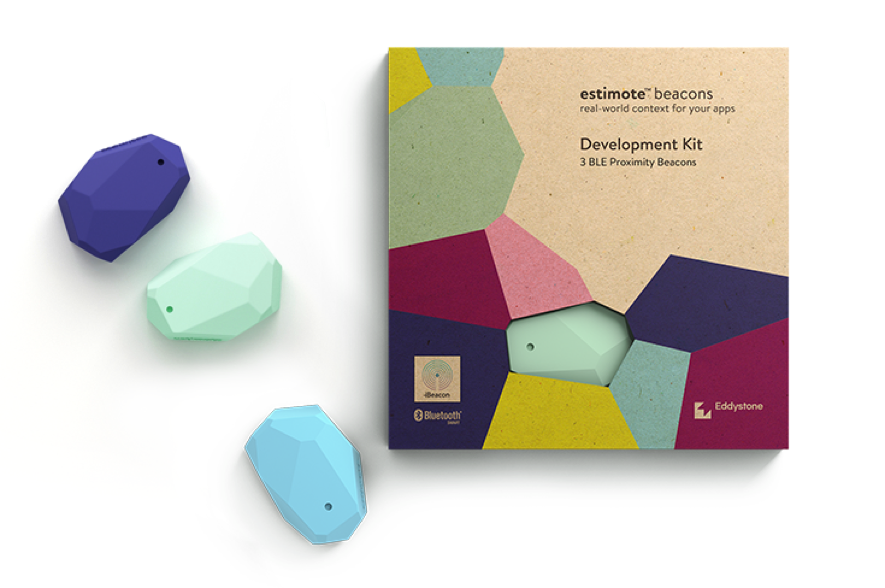
\includegraphics[width=0.6\textwidth]{Figures/estimote_data.png}
  \caption[Estimote Proximity Beacons]{Estimote Proximity Beacons.}
  \label{fig:estimotebeacon}
\end{figure}

They have received a lot of criticism related to their beacon’s battery, because once it is exhausted, the device becomes useless.
The Metropolitan Museum of Art, the Cleveland Museum of Art and the Solomon R. Guggenheim Museum in New York are some examples of users of the Estimote’s beacons.

\subsection{Gimbal} 
\label{subsection:gimbal}
Gimbal\footnote{http://www.gimbal.com} was incubated within Qualcomm, the largest producer of mobile semi-conductors in the world. 
The price of Gimbal hardware is very competitive because they charge a monthly active user fee due to the use of the available cloud service functionality that has to be used with their beacons' security protocol. Gimbal proximity beacon series 21 is introduced in Figure~\ref{fig:gimbalbeacon}.

\begin{figure}[!htb]
  \centering
  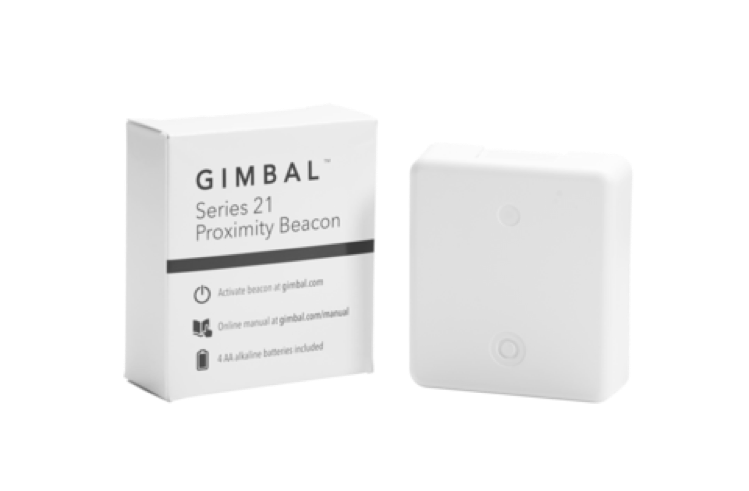
\includegraphics[width=0.6\textwidth]{Figures/gimbal_data.png}
  \caption[Gimbal Proximity Beacon Series 21]{Gimbal Proximity Beacon Series 21.}
  \label{fig:gimbalbeacon}
\end{figure}

This model may not be acceptable to solution builders who simply want high quality hardware and to create their own cloud platform to support a network strategy or a middleware offering. In this case, there may be some challenges in reconciling strategies.
Brands including GameStop and Major League Baseball are among Gimbal’s current customers.

\subsection{Kontakt.io} 
\label{subsection:kontakt}
Kontakt.io\footnote{https://kontakt.io} is an \gls{iot} company and they have focused on monetizing beacon hardware rather than charging for active users. Their image is rooted on cause-based solutions, with a founding story that relates to providing assistance for blind people with beacon-enabled mobile applications. 

The Kontakt.io hardware, shown in Figure~\ref{fig:kontaktbeacon}, is distinguished by a \gls{wi-fi} to Bluetooth gateway or cloud beacon and a robust weather-resistant tough beacon. There are limitations to their beacons’ power options. Their beacons rely on thick coin cell batteries, which limits the battery life to six months when broadcasting at Apple’s prescribed 100ms interval. 

\begin{figure}[!htb]
  \centering
  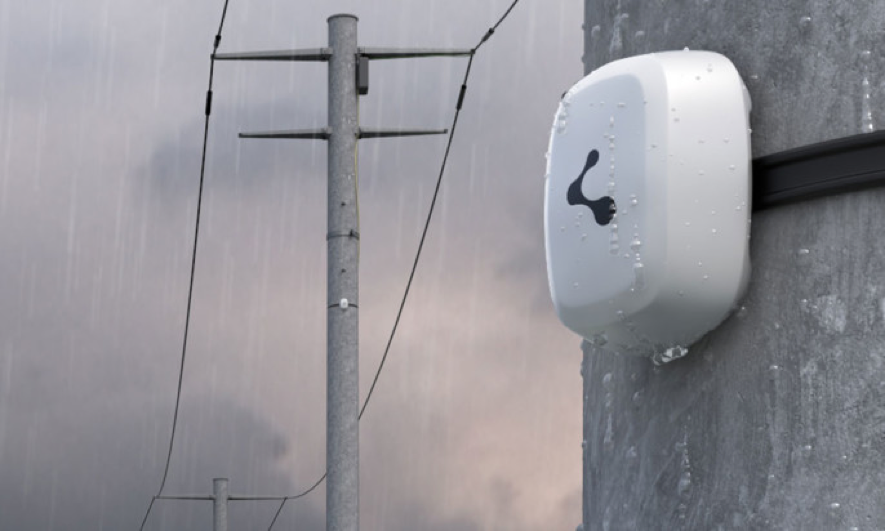
\includegraphics[width=0.6\textwidth]{Figures/kontakt_data.png}
  \caption[Kontakt Beacon]{Kontakt Beacon.}
  \label{fig:kontaktbeacon}
\end{figure}

McDonald’s have recently leveraged a new proximity marketing strategy at 15 McDonald's Cafés in Istanbul, Turkey, sending beacon-enabled promotions to customers within its venues via a mobile application, resulting in a conversion rate of 20 percent.

\subsection{Iotton} 
\label{subsection:iotton}
Iotton~\footnote{http://iotton.com} call themselves a Smart \gls{iot} Solution Provider. They have their headquarters in China and sell \gls{iot} solutions for the rest of the World from online sales sites.
Due to the location where the beacons are produced and their beacons' simple model, presented in Figure~\ref{fig:iottonbeacon}, Iotton can sell very low cost beacons, even if they often have to send the beacons far away, making the users pay for the shipment

\begin{figure}[!htb]
  \centering
  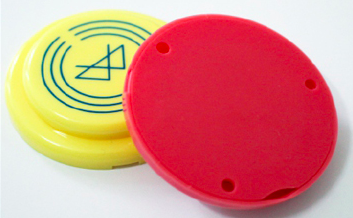
\includegraphics[width=0.4\textwidth]{Figures/iotton_data.png}
  \caption[Iotton's beacon tag]{Iotton's beacon tag.}
  \label{fig:iottonbeacon}
\end{figure}

\subsection{Shenzhen Sky Electronics Manufactory} 
\label{subsection:shenzhen}
Shenzhen Sky Electronics Manufactory is a manufacturer company with their headquarters in Guangdong, China. 
Their beacons have a visual very close to the Estimote beacons but they provide the user the possibility of removing the battery and replace it with a new one, which is an advantage. In Figure~\ref{fig:shenbeacon} it is possible to see how the battery can be removed.

\begin{figure}[!htb]
  \centering
  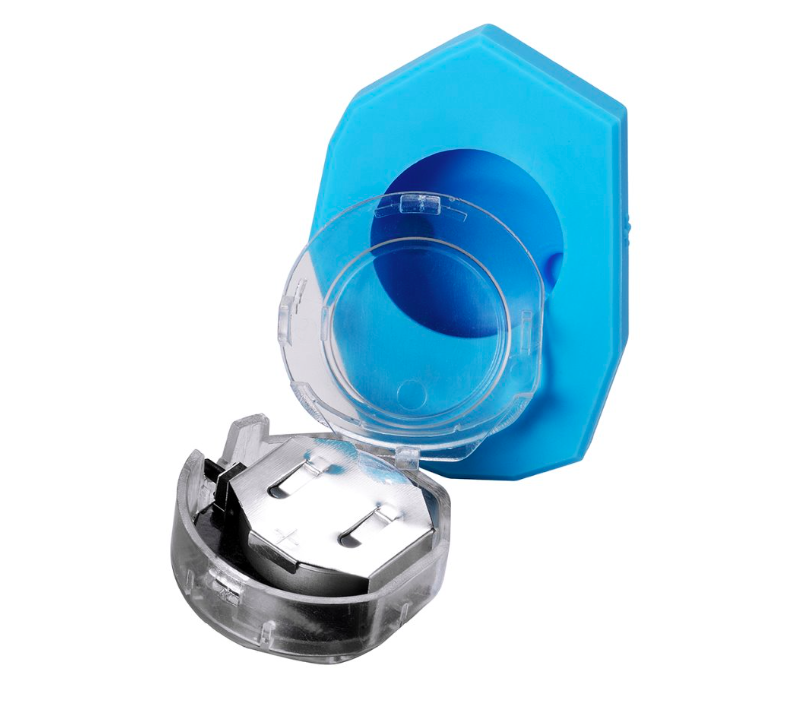
\includegraphics[width=0.5\textwidth]{Figures/shen_data.png}
  \caption[Shenzhen Sky Electronics Manufactory's beacon]{Shenzhen Sky Electronics Manufactory's beacon.}
  \label{fig:shenbeacon}
\end{figure}


\subsection{Comparison} 
\label{subsection:comparison1}

In short, it is possible to combine the characteristics of the beacons from the most known beacon manufacturers, such as: cost, range, battery life and if the battery is rechargeable or not. These features are compared in the Table~\ref{tab:manufdif}. 

\begin{table}[!htb]
  \renewcommand{\arraystretch}{1.5} % more space between rows
  \centering
  \resizebox*{\textwidth}{!}{
  \begin{tabular}{lccc p{1.5cm}}
    \toprule
   \textbf{ Beacons      } &Estimote Proximity Beacons&Gimbal Proximity Beacon Series 21&Kontakt.io Beacon\\
    \midrule
    \textbf{Manufacturer}    &Estimote&Gimbal&Kontakt.io \\
    \textbf{Price }			&\$59 - 3 beacons&\$30.00 - 1 beacon&\$60.00 - 3 beacons\\
    \textbf{Range}	&70m&50m&70m\\
    \textbf{Battery life}  &\begin{tabular}[t]{@{}c@{}}24 months, can change depending on\\ the use of their Smart Power Mode \end{tabular}&18 months, transmitting every 100ms&\begin{tabular}[t]{@{}c@{}}24 months transmitting every 350ms or\\ 6 months transmitting every 100ms\end{tabular}\\
    \textbf{Rechargeable	}	&No&Yes, four standard AA alkaline batteries&Yes\\
    \bottomrule
  \end{tabular}
  }
  \caption[Manufacturers' Beacons Differences]{Manufacturers' Beacons Differences.}
  \label{tab:manufdif}
\end{table}

It is possible to see that the Gimbal's beacon is more expensive than the others because when the user buys a Gimbal's beacon it grants access to their databases using Gimbal's Security Protocol, which requires a monthly fee.

Iotton's IonBeacon Ton9108 costs \$4.69 per unit and the shipment of 10 units with DHL express costs \$21.00 making the total cost of \$67.90, much lower than the cost done by the the manufacturers introduced before, even though it only differs in the battery life and the \gls{tx} interval. Iotton beacon only permits \gls{tx} intervals of 200ms, 300ms, 500ms and 900ms.

Shenzen's beacon costs \$8 per unit and the shipment of 10 units costs with DHL express \$18 making the total cost of \$98, much lower than the previous manufacturers with equivalent characteristics and with the possibility to replace the battery.

All of the manufacturers provide their \gls{api} to change the beacons' power intensity, their interval of \gls{tx} and their \gls{sdk} to the developers.

\section{Applications}
\label{section:aplications}

The market already has several applications related to the beacon positioning. However, most of these solutions can only be used to the purpose they were developed for and the application code is not open to the community. Some of these applications are:
\begin{itemize}
\item Launch Here;
\item Ballpark;
\item San Francisco International Airport.
\end{itemize}

\subsection{Launch Here}
\label{subsection:launchhere}
"Launch Here" application allows the user to automate tasks on its \gls{ios} devices.
Multiple beacons can be place in locals where the user opens the same application or a \gls{url} regularly, so that next time that the user approaches that beacon the Launch Here application will trigger an application or an \gls{url} which is associated with that beacon.

For example, if a beacon is placed near a sofa at home and the user comes near it , Launch Here can launch a journal application. The hour of this notification can be set before it is triggered so that no unwanted notifications happen.
To launch this application, the user needs to have an iBeacon.

As soon as the user is nearby a placed beacon and the screen is unlocked, the application of choice will appear as notification, shown in Figure~\ref{fig:lauchhereapp}, and a simple swipe can launch it.

\begin{figure}[!htb]
  \centering
  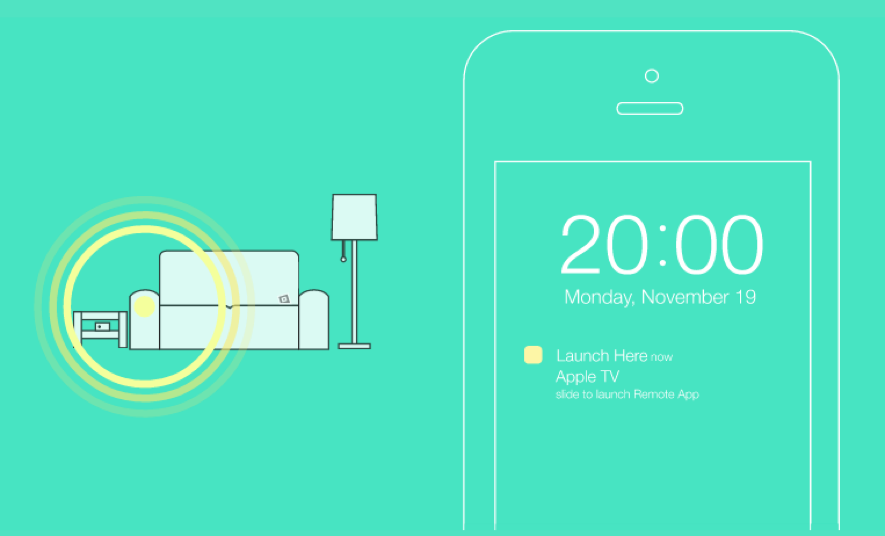
\includegraphics[width=0.6\textwidth]{Figures/launchhere_data.png}
  \caption[Lauch Here Application]{Launch Here Application.}
  \label{fig:lauchhereapp}
\end{figure}

\subsection{Ballpark}
\label{subsection:ballpark}
MLB.com Ballpark application\footnote{http://mlb.mlb.com/mobile/ballpark/}
%, shown in Figure~\ref{fig:ballparkapp}, 
is one of the best applications in the sports domain and has several interesting features, working as follows: when the user loads the application on the way to the stadium, it immediately identifies the stadium and opens information specific to that one. Once near the entrance, it displays the barcode of the user ticket and directs the user to the relevant seat via a map while also highlighting the nearby points of interest.

From the owner of the application point of view, the application can also track the visits made by their fans, enabling them to reward fans with special coupons and discounts for their frequent visits, shown in Figure~\ref{fig:ballparkapp}. 


\begin{figure}[!htb]
  \centering
 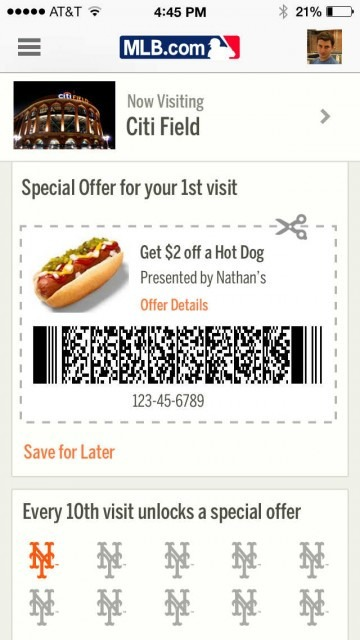
\includegraphics[width=0.35\linewidth]{Figures/ballpark3_data.png}
  \caption[At the Ballpark Application]{At the Ballpark Application.}
 \label{fig:ballparkapp}
\end{figure}


\subsection{San Francisco International Airport}
\label{subsection:sanfrancisco}
San francisco International Airport~\footnote{http://www.flysfo.com/pt} tested a way to help visually-impaired people to navigate around one of their terminals using beacons. These beacons are provided by Indoo.rs an indoor positioning company.
The system uses Apple's Voiceover technology to read out points of interest as they come on screen, meaning that the application could read in the display how to move to the nearest point of interest that appears in the application. In Figure \ref{fig:sanfranapp} a map can be seen in the mobile device.

\begin{figure}[!htb]
  \centering
  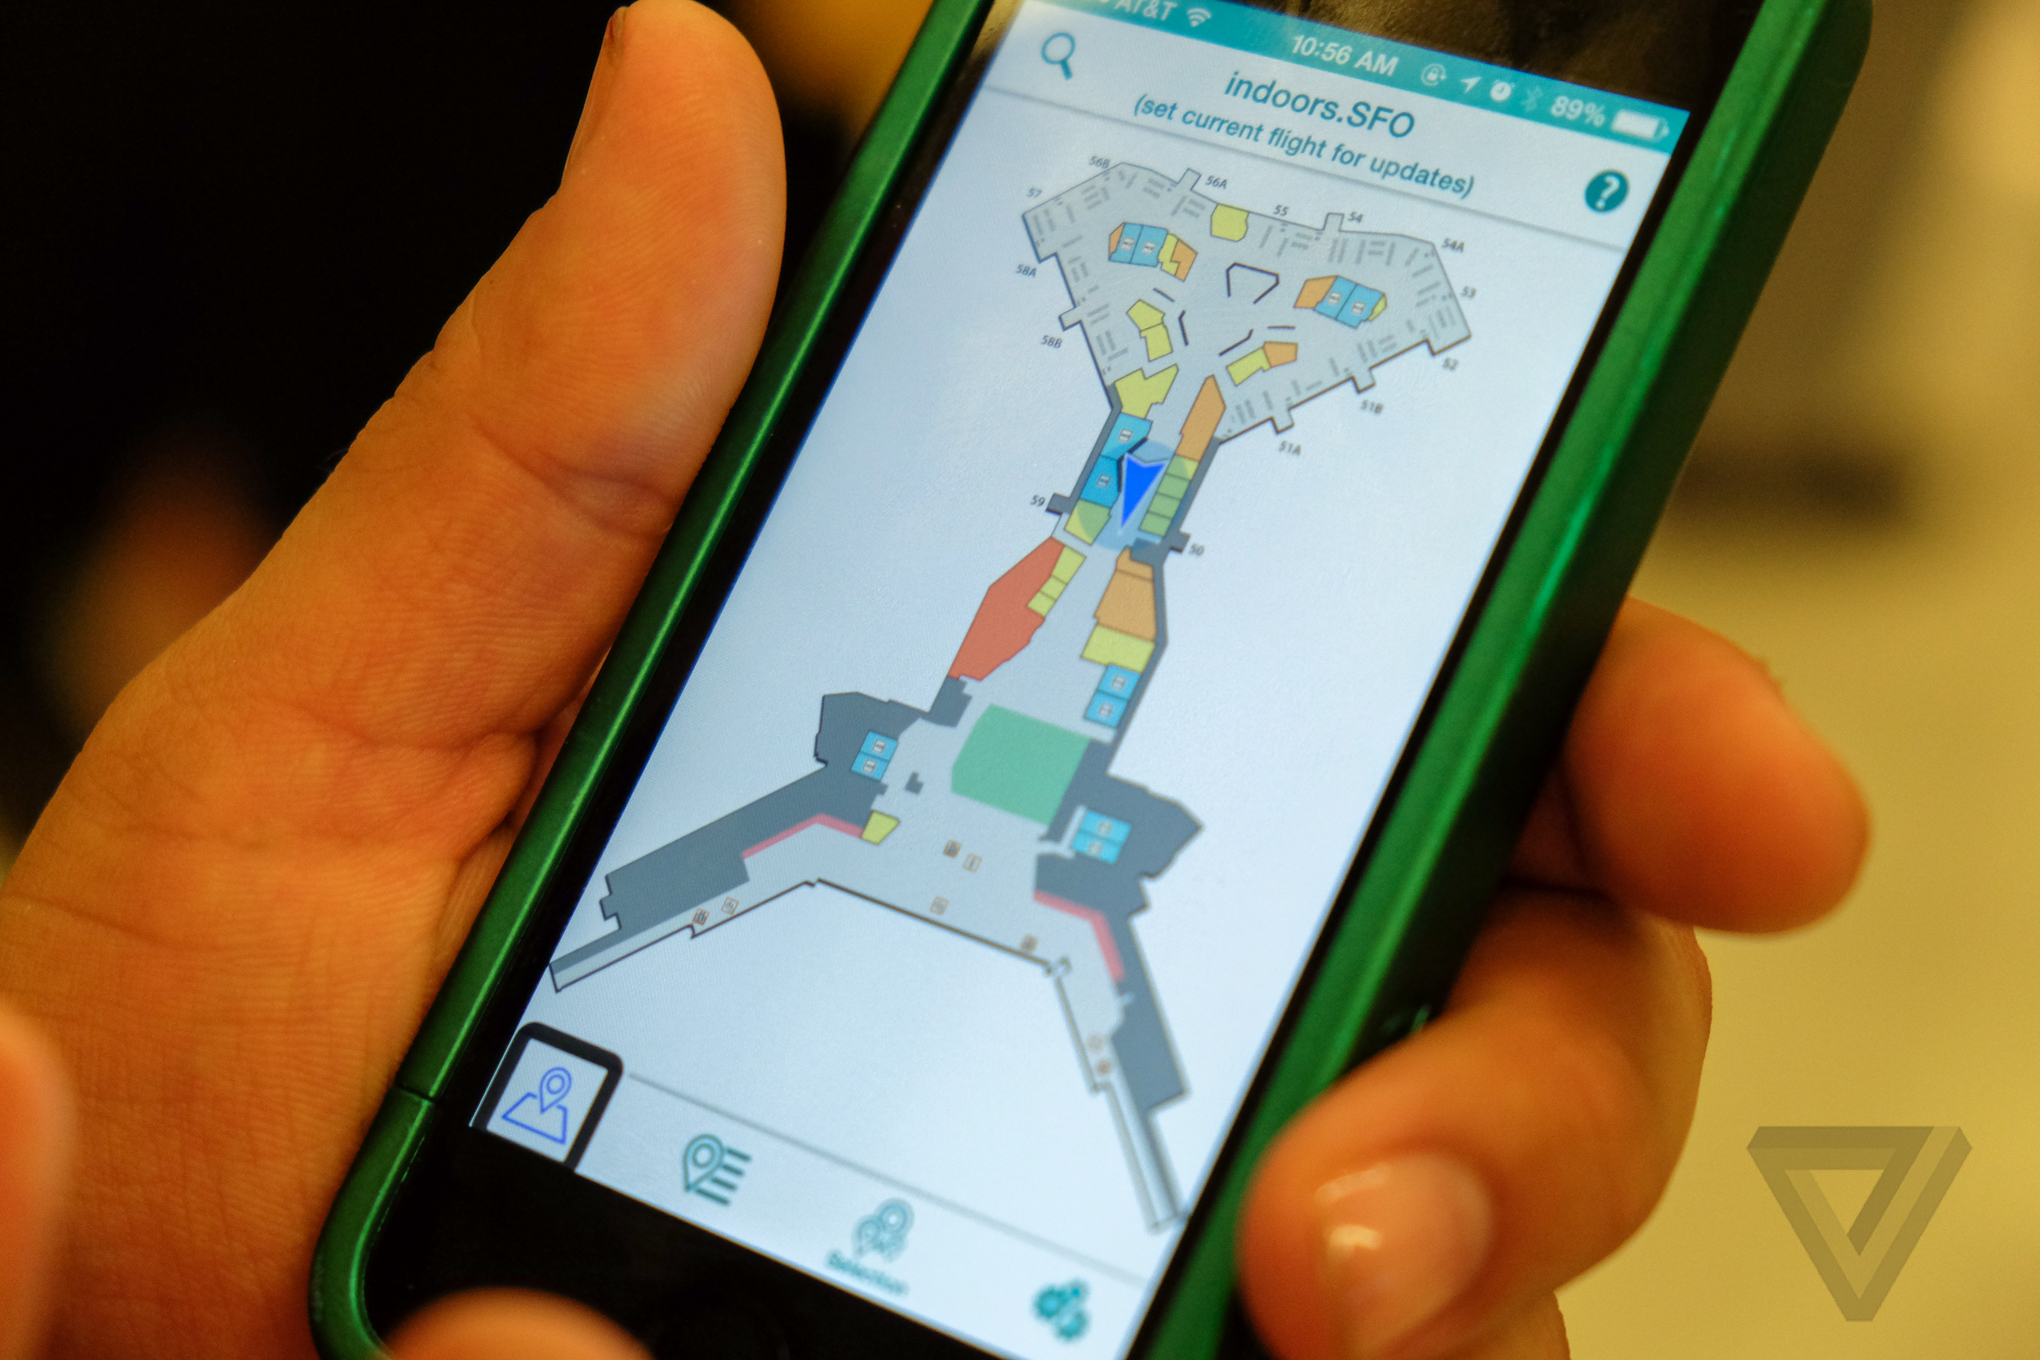
\includegraphics[width=0.6\textwidth]{Figures/sanfrancisco_data.jpg}
  \caption[San Francisco International Airport Map]{San Francisco International Airport Application.}
  \label{fig:sanfranapp}
\end{figure}


In general the applications using beacons are being used to provide the users with the latest promotions or relevant information and welcome them as they enter the owner's store, museum, hospital, restaurant, airport, stadium, etc. 
To the owner of the beacons application, it can inform them where their customers have been, keeping track of them.



\section{Summary}
\label{section:summarybackground}
%%%%%%%%%%%%%%%%%%%
In order to create an indoor system to estimate the position of a mobile device, technologies and methods need to be used or implemented. Cost, accuracy, precision, complexity, scalability and robustness are variables in a technology. \gls{gps}, \gls{wi-fi}, Bluetooth, \gls{qrcodes}, \gls{nfc} and \gls{rfid} are introduced presenting their differences relating the variables mentioned before and their limitations in an indoor environment. \gls{gps} is unsuitable for indoor positioning due to its low accuracy and precision. In some mobile devices is impossible to access the value of \gls{rss} from all access points in the range of the mobile device, making \gls{wi-fi} impossible to use more advanced positioning methods. Bluetooth has a delay due to the transmission intervals of the \gls{ble} devices or beacons. \gls{qrcodes}, \gls{nfc} and \gls{rfid} need the user to be aware of them. 

The measured \gls{rss} can be used to calculate the position of a device using the Friis free space model Equation.
Positioning methods can be active or passive. Active positioning methods determine the position of a device based on the signals received. Proximity sensing, lateration and angulation are all active positioning methods. Passive positioning methods depend in the environment. Fingerprinting is a passive positioning method.

Beacons work following a protocol. iBeacon, AltBeacon, Eddystone and URIBeacon are beacon' protocols. These protocols differ in the advertisement format. iBeacon and AltBeacon broadcast a unique ID number. URIBeacon broadcasts and \gls{url}. Eddystone can broadcast both an ID number or an \gls{url}.

Beacons' manufacturers try to differentiate among others presenting different physical aspects in their hardware, in their software, or in the business aspects that they offer to the user's solutions. Estimote, Gimbal and Kontakt are some of the most well-known manufacturers. They differ in the appearance of their beacons, their battery life and its rechargeability. They offer to their development clients different \gls{sdk}s. Estimote and Kontakt are more common inside developers. Iotton and Shenzhen Sky Eletronics are the cheapest choice when it comes to a beacons solution.

Applications are being developed to welcome the clients by using Bluetooth beacons. To the owner, these beacons can mean the possibility of keeping track of the customers. To the customers, these beacons can represent the possibility of receiving the latest promotions or information relevant to the place where they position.
 % file "Thesis_Background.tex"
%\cleardoublepage

\chapter{Design Choices}
\label{chapter:designchoices}

In the implementation of any positioning system, it is necessary to choose the hardware and software required to realize it. 
Having in mind what was discussed in Chapter~\ref{chapter:background} and taking into consideration other requirements, namely availability and financial restrictions, we decided to choose the Bluetooth technology, \gls{ble}, using the protocol iBeacon for the beacon information broadcasting. iBeacon only broadcasts an \gls{uuid}, so the positioning system needs a back-end to support the information that the mobile phone application receives. Back-end is accessed through the application via \gls{wi-fi}/ 3G or directly accessed to collect the data. The architecture can be divided in 3 components: beacons, mobile phone application, information system (back-end), in Figure~\ref{fig:motiv} a visual description is given.

%\begin{figure}[!htb]
%	\centering
%	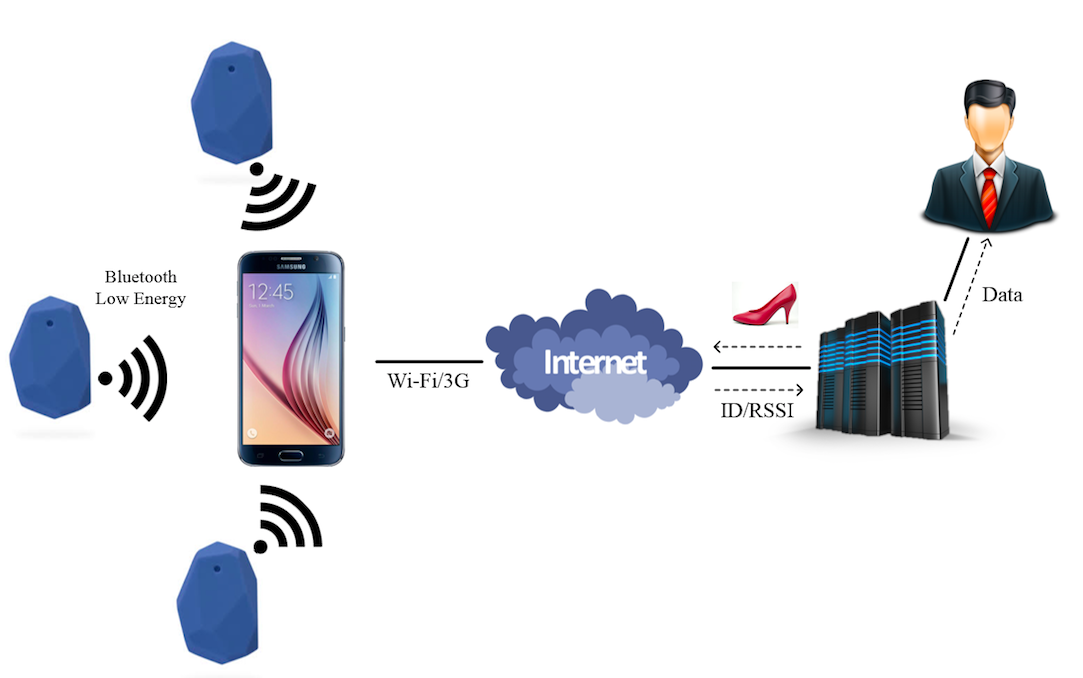
\includegraphics[width=0.9\textwidth]{Figures/architecture.png}
%	\caption[Architecture]{Architecture.}
%	\label{fig:architecture}
%\end{figure}


\section{Beacons}
\label{section:beaconsdesign}

The chosen beacons, due to its battery life and four different values of power intensity, are the ones manufactured by \textit{Shenzen Sky Eletronics Manufactory}.

In order to achieve better results in the calculation of the user's position, beacons must be placed as high as possible since height maximizes coverage of an area and minimizes the attenuation and signal fluctuations that comes from signals being absorbed by people’s bodies. However, if the beacon is too high, geometry starts to work against it, especially if the system is a very localized proximity trigger. Added to this, a higher placement also has the inevitable consequence that it requires ladders or elevated platforms for battery change or a reboot~\citep{Statler}. In Figure~\ref{fig:placement} one can see an example of a local with beacons.

%Escolhemos estes que consequencia têm e apresentar quantidades para area...
When deploying the beacons, there are many parameters to consider, such as: algorithm construction, beacon rate, transmit power, beacon mobility, beacon geometry, beacon density, etc. Performing an exhaustive search of parameter space involves constant beacon redeployment and the result would be highly environment specific. A dense beacon distribution has 1 beacon per 30 $m^{2}$ and a lower density distribution, 1 beacon per 100 $m^{2}$ ~\citep{fingerprintingble}.

\begin{figure}[!htb]
	\centering
	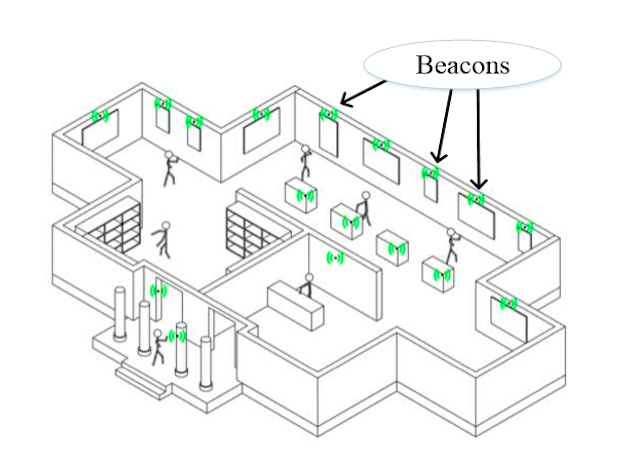
\includegraphics[width=0.9\textwidth]{Figures/placementv2.png}
	\caption[Beacons placement]{Beacons placement.}
	\label{fig:placement}
\end{figure}




\section{Mobile phone Application}
\label{section:app}
The mobile phone application is used by the customer, so it needs to be
user-friendly with an appealing look. When started, the application shows the logotype of the information system and its name. Furthermore, the application shows useful information related to a product or local, links, description or barcodes, Figure~\ref{fig:app_logo} is a template.

\begin{figure}[!htb]
	\centering
	\begin{subfigmatrix}{2}
	\subfigure[Logo]{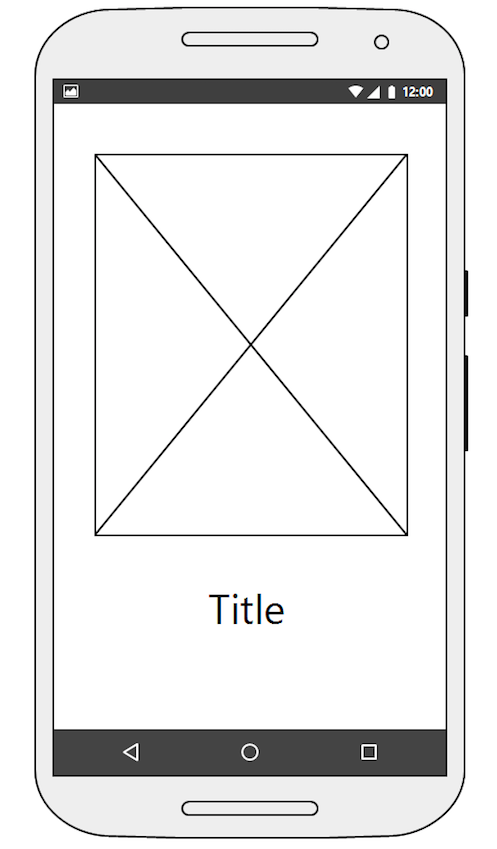
\includegraphics[width=0.35\linewidth]{Figures/logo.png}}
	\subfigure[Product]{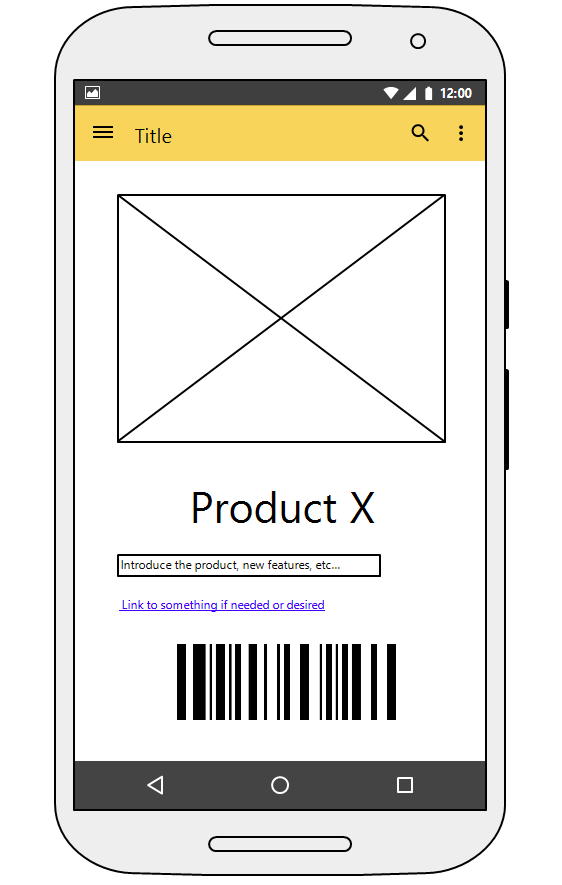
\includegraphics[width=0.38\linewidth]{Figures/product.png}}
	\end{subfigmatrix}
	\caption[Logo and product activities]{Logo and product activities.}
	\label{fig:app_logo}
\end{figure}


Application may have several user profiles, and because of that it can made the sign up and the sign in of the users. These user profiles can be used to save the user's interest or where he has been previously.


\begin{figure}[!htb]
	\centering
	\begin{subfigmatrix}{2}
		\subfigure[Sign up]{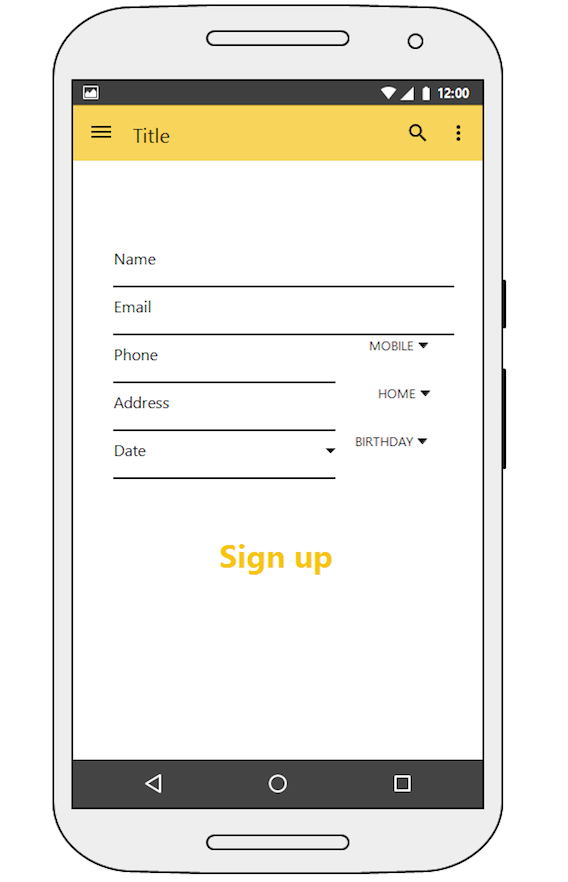
\includegraphics[width=0.39\linewidth]{Figures/signup.png}}
		\subfigure[Sign in]{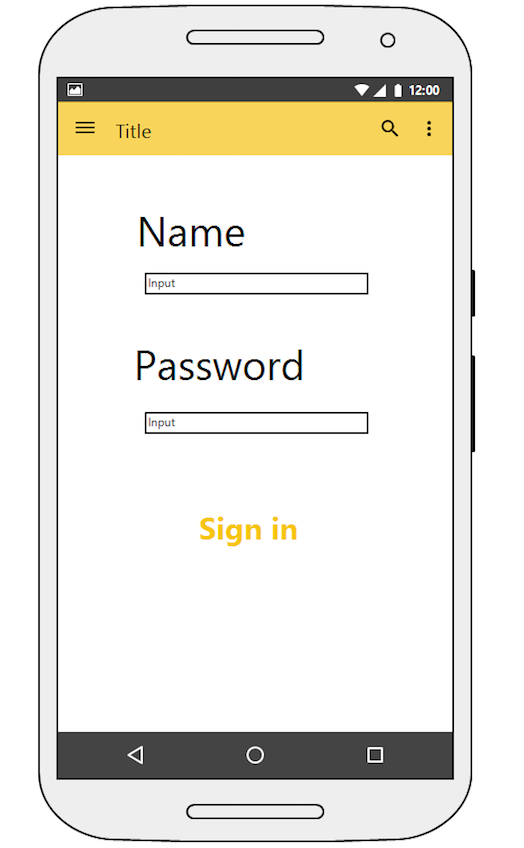
\includegraphics[width=0.37\linewidth]{Figures/signin.png}}
	\end{subfigmatrix}
	\caption[Sign Activities]{Sign Activities.}
	\label{fig:app_sign}
\end{figure}

After, the user is presented with a menu with all the important items or information. Selecting one of them directs the user to its page. In addition to the option to view the list of items, it is also possible to see a map of the location of those items and the user's location, which changes according to his or her position. If the user is close to a specific item, a notification is issued informing the user about the relevant information pertinent to the item . By selecting this notification, it opens an activity to the item information, as shown in Figure~\ref{fig:app_logo}. It should be possible to disable these notifications in the tools button localized in the action bar.


\begin{figure}[!htb]
	\centering
	\begin{subfigmatrix}{2}
		\subfigure[Products list]{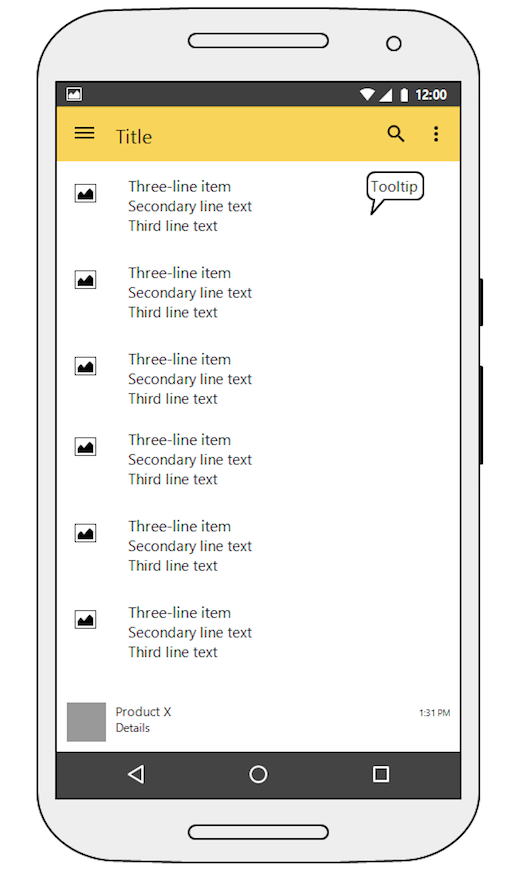
\includegraphics[width=0.35\linewidth]{Figures/list.png}}
		\subfigure[Map]{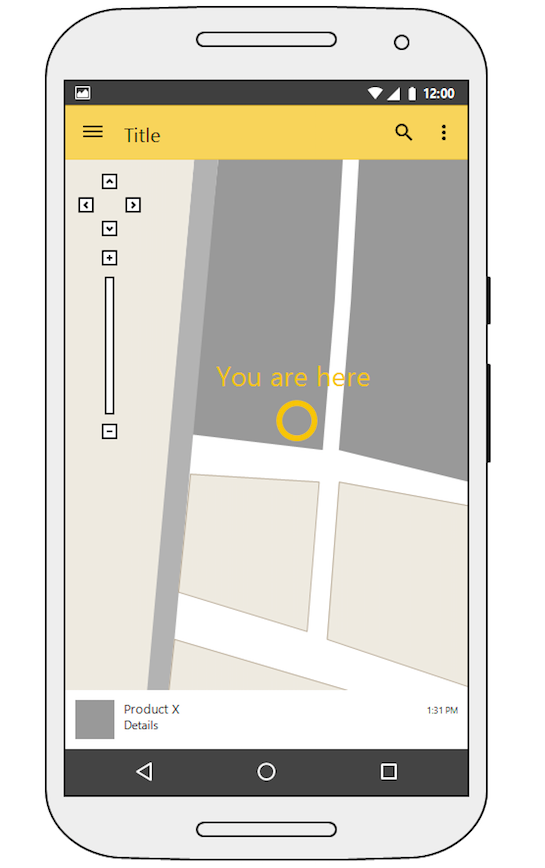
\includegraphics[width=0.38\linewidth]{Figures/map.png}}
	\end{subfigmatrix}
	\caption[Itmes list and Map activities]{Items list and Map activities.}
	\label{fig:app_menu}
\end{figure}

The activities are interconnected and from the first activity it should be possible to move to the register or to the list of items, depending if the user has already signed in. It should be possible to reach the item through the map, notifications or the list.
Figure~\ref{fig:app_story} demonstrates the connection between the activities. The application may send notifications to the user even if it is put in background.
\begin{figure}[!htb]
	\centering
	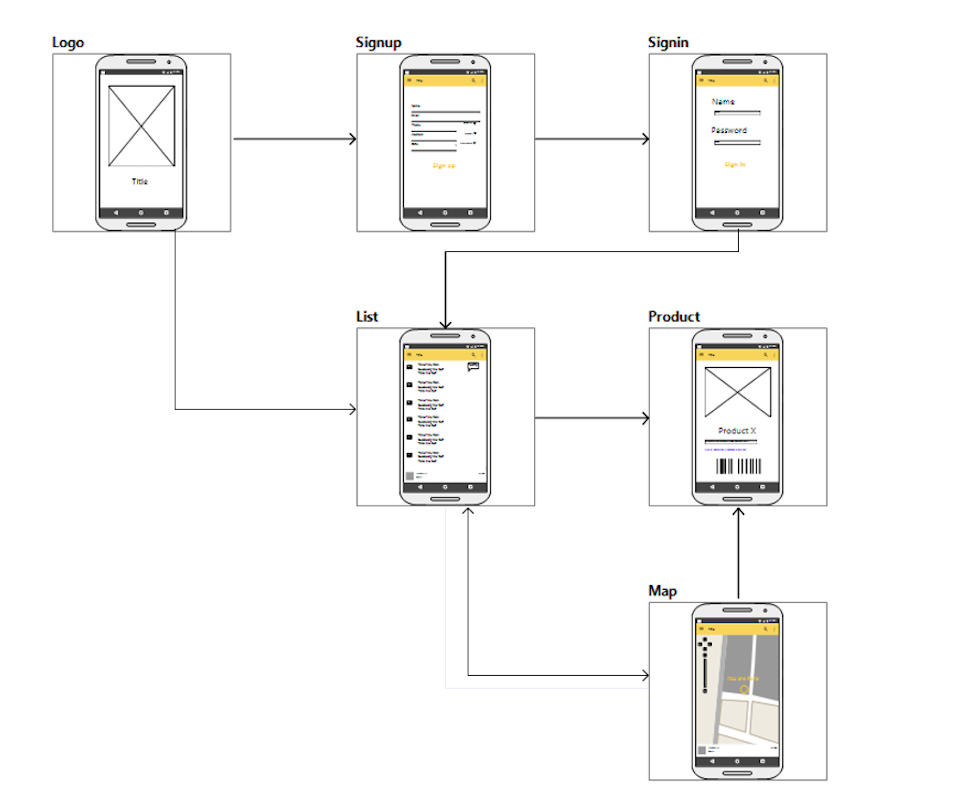
\includegraphics[width=0.85\textwidth]{Figures/story.png}
	\caption[Mobile phone application story]{Mobile phone application story.}
	\label{fig:app_story}
\end{figure}

\section{Back-end}
\label{section:backend}

The back-end has two parts in it: server and database.
The back-end stores all the information related to the user's presence, storing the \gls{rssi} and \gls{uuid} received from the user as well as the accompanying timestamps. It also keeps track of which items the user has selected in the application. This information can be saved in the user profile, if the sign in has been made, or / and saved with the mac address of the user's mobile phone.
It has the map information about the store and where are the items in it.
It has the images of all items and the information that is related to these. 
It responds to the application requests, for updates of the images or description of certain items.
Furthermore, the system owner can access the data collected by the server that is in the database and see this data in an Excel sheet or in a program previously prepared for that task.

Depending on context items can be different things. For instance in a store, items can be products or classes of products, on a museum items can be artworks, on hospitals items can be related to specific areas of expertise. 

\section{Implementation Scenarios}
\label{section:scenarios}
The implementation of the positioning system has two possible scenarios. In the first scenario, we will build a mock-up of context at \gls{ist}, in order to make artificial tests and change the location of the beacons more easily. In the second scenario, we expect to reach an agreement with a commercial enterprise to place the beacons within a location to be defined. FNAC is a possibility since it has a small store at \gls{ist}, but may be open to the implementation of such a setup in a more general setting.

\section{Summary}
\label{section:summary}

The positioning system consists in 3 components: beacons, mobile phone application and back-end. 

The beacons broadcast their \gls{uuid} using the iBeacon protocol. The application listens and collects the \gls{uuid} and their \gls{rssi} and using these the application calculate its position. Then the application sends, from time to time, the user's position to the back-end where it collects the data, recomputes necessary information and sends updates back to the application. The application can have different customer profiles displaying only the information related to the user profile. In the application, the user should have access to a map and a list of all items. The data in the back-end can be accessed by the owner or administrator of the system.

The implementation of the system will have two different scenarios. Initially, the system is deployed at \gls{ist} to make tests. After, the system will be deployed at some store agreed with vendor. % file "Thesis_Implementation.tex"
%\cleardoublepage

\chapter{Thesis' Planning}
\label{chapter:planning}

The planned work to be continued after the end of \textit{Introduction to the Research in Electrical and Computer Engineering} is represented in Figure~\ref{fig:gantt}.

\begin{figure}[!htb]
	\centering
	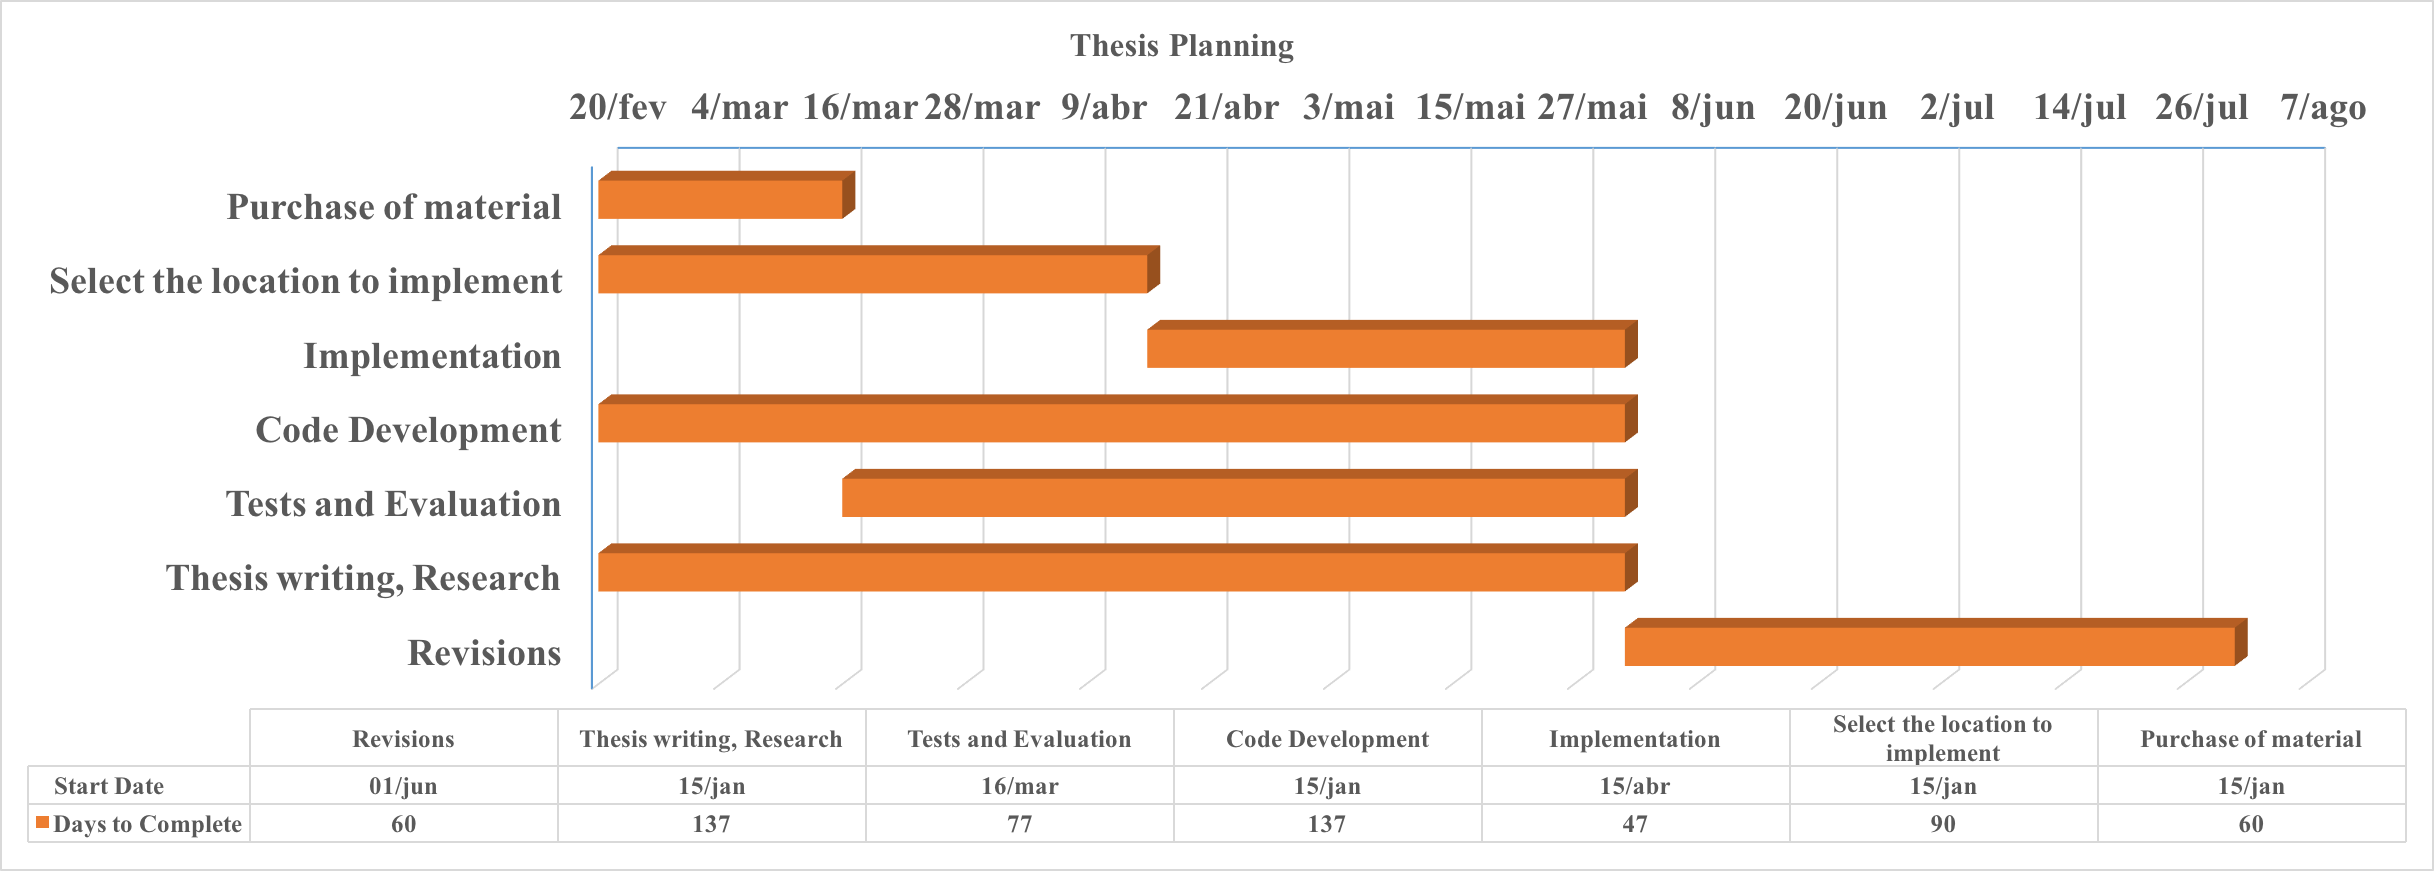
\includegraphics[width=1\textwidth]{Figures/gantt_v2.png}
	\caption[Gantt Diagram]{Gantt diagram.}
	\label{fig:gantt}
\end{figure}

Currently, we have already started the process of purchase of the necessary material, more specifically the Bluetooth beacons, and plan where to implement the positioning system. In addition to these two tasks, the code to perform the algorithm (Lateration~(\ref{subsection:lateration}) and/or Fingerprinting~(\ref{subsection:fingerprinting})) and the communication between the mobile phone application (\ref{section:app}) and the back-end (\ref{section:backend}) will be developed. After receiving the beacons, code related to these, such as beacon detection and acquirement of their \gls{rssi} and \gls{uuid} by the application, will be developed and tested in the first scenario nominative in Section~\ref{section:scenarios}.

As soon as the place to implement the system is chosen, the implementation starts in the second scenario indicated in~\ref{section:scenarios}, making at the same time, if needed, changes in the code or bug fixes.

The writing of the thesis will be carried out during the course of the tasks described previously. Implementation, Evaluation and Conclusion will be developed and finalized as the work progresses.

After the completion of these tasks, a review time is provided to make unexpected changes.

Delivery is estimated to be between June 1 and July 31. The discussion of the thesis must be performed after the delivery of the same, sometime no later than October.
 % add new .tex files for new chapters
% \cleardoublepage

%\input{Thesis_new_file} % add new .tex files for new chapters
% \cleardoublepage

%\input{Thesis_new_file} % add new .tex files for new chapters
% \cleardoublepage

%%%%%%%%%%%%%%%%%%%%%%%%%%%%%%%%%%%%%%%%%%%%%%%%%%%%%%%%%%%%%%%%%%%%%%%%%
%                                                                      %
%     File: Thesis_Results.tex                                         %
%     Tex Master: Thesis.tex                                           %
%                                                                      %
%     Author: Andre C. Marta                                           %
%     Last modified :  2 Jul 2015                                      %
%                                                                      %
%%%%%%%%%%%%%%%%%%%%%%%%%%%%%%%%%%%%%%%%%%%%%%%%%%%%%%%%%%%%%%%%%%%%%%%%

\chapter{Results}
\label{chapter:results}

Insert your chapter material here...


%%%%%%%%%%%%%%%%%%%%%%%%%%%%%%%%%%%%%%%%%%%%%%%%%%%%%%%%%%%%%%%%%%%%%%%%
\section{Problem Description}
\label{section:problem}

Description of the baseline problem...


%%%%%%%%%%%%%%%%%%%%%%%%%%%%%%%%%%%%%%%%%%%%%%%%%%%%%%%%%%%%%%%%%%%%%%%%
\section{Baseline Solution}
\label{section:baseline}

Analysis of the baseline solution...


%%%%%%%%%%%%%%%%%%%%%%%%%%%%%%%%%%%%%%%%%%%%%%%%%%%%%%%%%%%%%%%%%%%%%%%%
\section{Enhanced Solution}
\label{section:enhanced}

Quest for the optimal solution...


% ----------------------------------------------------------------------
\subsection{Figures}
\label{subsection:figures}

Insert your section material and possibly a few figures...

Make sure all figures presented are referenced in the text!


% ----------------------------------------------------------------------
\subsubsection{Images}
\label{subsection:images}

\begin{figure}[!htb]
  \centering
  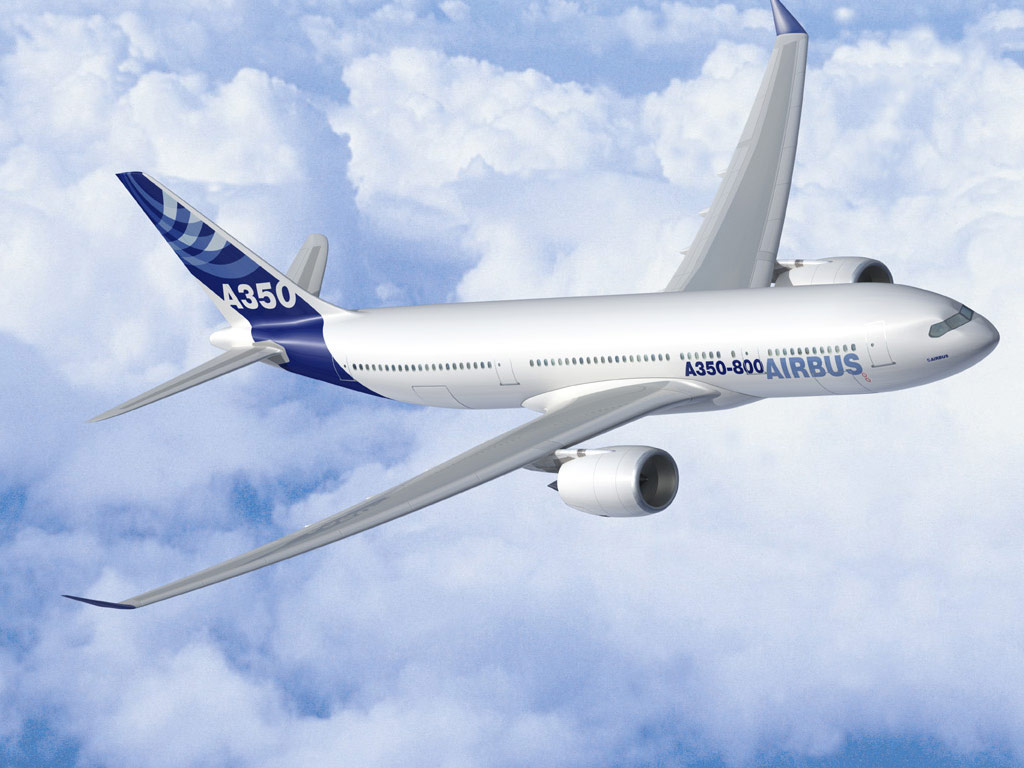
\includegraphics[width=0.25\textwidth]{Figures/Airbus_A350.jpg}
  \caption[Caption for figure in TOC.]{Caption for figure.}
  \label{fig:airbus1}
\end{figure}

\begin{figure}[!htb]
  \begin{subfigmatrix}{2}
    \subfigure[Airbus A320]{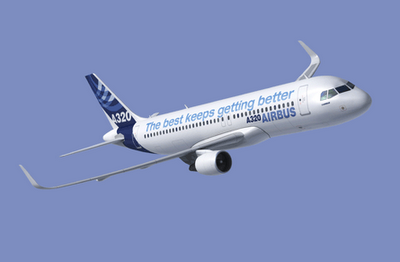
\includegraphics[width=0.49\linewidth]{Figures/Airbus_A320_sharklets.png}}
    \subfigure[Bombardier CRJ200]{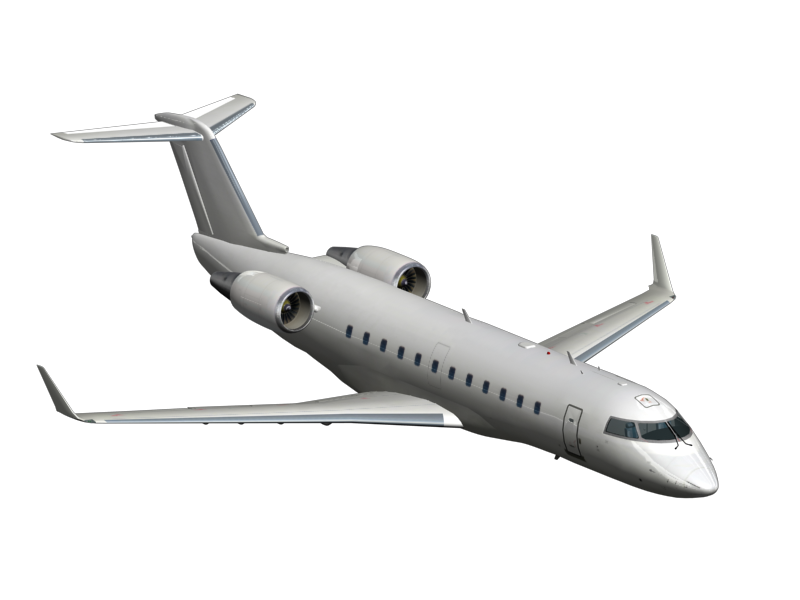
\includegraphics[width=0.49\linewidth]{Figures/Bombardier_CRJ200.png}}
  \end{subfigmatrix}
  \caption{Some aircrafts.}
  \label{fig:aircrafts}
\end{figure}

Make reference to Figures \ref{fig:airbus1} and \ref{fig:aircrafts}.

By default, the supported file types are {\it .png,.pdf,.jpg,.mps,.jpeg,.PNG,.PDF,.JPG,.JPEG}.

See \url{http://mactex-wiki.tug.org/wiki/index.php/Graphics_inclusion} for adding support to other extensions.


% ----------------------------------------------------------------------
\subsubsection{Drawings}
\label{subsection:drawings}

Insert your subsection material and for instance a few drawings...

The schematic illustrated in Fig.~\ref{fig:algorithm} can represent some sort of algorithm.

\begin{figure}[!htb]
  \centering
  \scriptsize
%  \footnotesize 
%  \small
  \setlength{\unitlength}{0.9cm}
  \begin{picture}(8.5,6)
    \linethickness{0.3mm}

    \put(3,6){\vector(0,-1){1}}
    \put(3.5,5.4){$\bf \alpha$}
    \put(3,4.5){\oval(6,1){}}
    %\put(0,4){\framebox(6,1){}}
    \put(0.3,4.4){Grid Generation: \quad ${\bf x} = {\bf x}\left({\bf \alpha}\right)$}

    \put(3,4){\vector(0,-1){1}}
    \put(3.5,3.4){$\bf x$}
    \put(3,2.5){\oval(6,1){}}
    %\put(0,2){\framebox(6,1){}}
    \put(0.3,2.4){Flow Solver: \quad ${\cal R}\left({\bf x},{\bf q}\left({\bf x}\right)\right) = 0$}

    \put(6.0,2.5){\vector(1,0){1}}
    \put(6.4,3){$Y_1$}

    \put(3,2){\vector(0,-1){1}}
    \put(3.5,1.4){$\bf q$}
    \put(3,0.5){\oval(6,1){}}
    %\put(0,0){\framebox(6,1){}}
    \put(0.3,0.4){Structural Solver: \quad ${\cal M}\left({\bf x},{\bf q}\left({\bf x}\right)\right) = 0$}

    \put(6.0,0.5){\vector(1,0){1}}
    \put(6.4,1){$Y_2$}

    %\put(7.8,2.5){\oval(1.6,5){}}
    \put(7.0,0){\framebox(1.6,5){}}
    \put(7.1,2.5){Optimizer}
    \put(7.8,5){\line(0,1){1}}
    \put(7.8,6){\line(-1,0){4.8}}
  \end{picture}
  \caption{Schematic of some algorithm.}
  \label{fig:algorithm}
\end{figure}


% ----------------------------------------------------------------------
\subsection{Equations}
\label{subsection:equations}

Equations can be inserted in different ways.

The simplest way is in a separate line like this

\begin{equation}
  \frac{{\rm d} q_{ijk}}{{\rm d} t} + {\cal R}_{ijk}({\bf q}) = 0 \,.
\label{eq:ode}
\end{equation}

If the equation is to be embedded in the text. One can do it like this ${\partial {\cal R}}/{\partial {\bf q}}=0$.

It may also be split in different lines like this

\begin{eqnarray}
  {\rm Minimize}   && Y({\bf \alpha},{\bf q}({\bf \alpha}))            \nonumber           \\
  {\rm w.r.t.}     && {\bf \alpha} \,,                                 \label{eq:minimize} \\
  {\rm subject~to} && {\cal R}({\bf \alpha},{\bf q}({\bf \alpha})) = 0 \nonumber           \\
                   &&       C ({\bf \alpha},{\bf q}({\bf \alpha})) = 0 \,. \nonumber
\end{eqnarray}

It is also possible to use subequations. Equations~\ref{eq:continuity}, \ref{eq:momentum} and \ref{eq:energy} form the Naver--Stokes equations~\ref{eq:NavierStokes}.

\begin{subequations}
    \begin{equation}
    \frac{\partial \rho}{\partial t} + \frac{\partial}{\partial x_j}\left( \rho u_j \right) = 0 \,,
    \label{eq:continuity}
    \end{equation}
    \begin{equation}
    \frac{\partial}{\partial t}\left( \rho u_i \right) + \frac{\partial}{\partial x_j} \left( \rho u_i u_j + p \delta_{ij} - \tau_{ji} \right) = 0, \quad i=1,2,3 \,,
    \label{eq:momentum}
    \end{equation}
    \begin{equation}
        \frac{\partial}{\partial t}\left( \rho E \right) + \frac{\partial}{\partial x_j} \left( \rho E u_j + p u_j - u_i \tau_{ij} + q_j \right) = 0 \,.
    \label{eq:energy}
    \end{equation}
\label{eq:NavierStokes}%
\end{subequations}


% ----------------------------------------------------------------------
\subsection{Tables}
\label{section:tables}

Insert your subsection material and for instance a few tables...

Make sure all tables presented are referenced in the text!

Follow some guidelines when making tables:

\begin{itemize}
  \item Avoid vertical lines
  \item Avoid “boxing up” cells, usually 3 horizontal lines are enough: above, below, and after heading
  \item Avoid double horizontal lines
  \item Add enough space between rows
\end{itemize}

\begin{table}[!htb]
  \renewcommand{\arraystretch}{1.2} % more space between rows
  \centering
  \begin{tabular}{lccc}
    \toprule
    Model           & $C_L$ & $C_D$ & $C_{M y}$ \\
    \midrule
    Euler           & 0.083 & 0.021 & -0.110    \\
    Navier--Stokes  & 0.078 & 0.023 & -0.101    \\
    \bottomrule
  \end{tabular}
  \caption[Table caption shown in TOC.]{Table caption.}
  \label{tab:aeroCoeff}
\end{table}

Make reference to Table \ref{tab:aeroCoeff}.

Tables \ref{tab:memory} and \ref{tab:multipleColumns} are examples of tables with merging columns:

\begin{table}[!htb]
  \renewcommand{\arraystretch}{1.2} % more space between rows
  \centering
  \begin{tabular}[]{lrr}
    \toprule
                & \multicolumn{2}{c}{\underline{Virtual memory [MB]}} \\
                & Euler       & Navier--Stokes \\
    \midrule
      Wing only &  1,000      &    2,000       \\
      Aircraft  &  5,000      &   10,000       \\
      (ratio)   & $5.0\times$ & $5.0\times$    \\
    \bottomrule
  \end{tabular}
  \caption{Memory usage comparison (in MB).}
  \label{tab:memory}
\end{table}

\begin{table}[!htb]
  \centering
  \renewcommand{\arraystretch}{1.2} % more space between rows
  \begin{tabular}{@{}rrrrcrrr@{}} % remove space to the vertical edges @{}...@{}
    \toprule
      & \multicolumn{3}{c}{$w = 2$} & \phantom{abc} & \multicolumn{3}{c}{$w = 4$} \\
    \cmidrule{2-4}
    \cmidrule{6-8}
      & $t=0$ & $t=1$ & $t=2$ && $t=0$ & $t=1$ & $t=2$ \\
    \midrule
      $dir=1$
      \\
      $c$ &  0.07 &  0.16 &  0.29 &&  0.36 &  0.71 &   3.18 \\
      $c$ & -0.86 & 50.04 &  5.93 && -9.07 & 29.09 &  46.21 \\
      $c$ & 14.27 &-50.96 &-14.27 && 12.22 &-63.54 &-381.09 \\
      $dir=0$
      \\
      $c$ &  0.03 &  1.24 &  0.21 &&  0.35 & -0.27 &  2.14 \\
      $c$ &-17.90 &-37.11 &  8.85 &&-30.73 & -9.59 & -3.00 \\
      $c$ &105.55 & 23.11 &-94.73 &&100.24 & 41.27 &-25.73 \\
    \bottomrule
  \end{tabular}
  \caption{Another table caption.}
  \label{tab:multipleColumns}
\end{table}

An example with merging rows can be seen in Tab.\ref{tab:multipleRows}.

\begin{table}[!htb]
  \renewcommand{\arraystretch}{1.2} % more space between rows
  \centering
  \begin{tabular}{ccccc}
    \toprule
      \multirow{2}{*}{ABC} & \multicolumn{4}{c}{header} \\
      \cmidrule{2-5} & 1.1 & 2.2 & 3.3 & 4.4 \\
    \midrule
      \multirow{2}{*}{IJK} & \multicolumn{2}{c}{\multirow{2}{*}{group}} & 0.5 & 0.6 \\
      \cmidrule{4-5}       & \multicolumn{2}{c}{}                       & 0.7 & 1.2 \\
    \bottomrule
  \end{tabular}
  \caption{Yet another table caption.}
  \label{tab:multipleRows}
\end{table}

If the table has too many columns, it can be scaled to fit the text widht, as in Tab.\ref{tab:scale}.
\begin{table}[!htb]
  \renewcommand{\arraystretch}{1.2} % more space between rows
  \centering
  \resizebox*{\textwidth}{!}{%
    \begin{tabular}[]{lcccccccccc}
      \toprule
        Variable &  a  &  b  &  c  &  d  &  e  &  f  &  g  &  h  &  i  &  j  \\
      \midrule
        Test 1   &  10,000 &  20,000 &  30,000 &  40,000 &  50,000 &  60,000 &  70,000 &  80,000 &  90,000 & 100,000 \\
        Test 2   &  20,000 &  40,000 &  60,000 &  80,000 & 100,000 & 120,000 & 140,000 & 160,000 & 180,000 & 200,000 \\
      \bottomrule
    \end{tabular}
  }%
  \caption{Very wide table.}
  \label{tab:scale}%
\end{table}


% ----------------------------------------------------------------------
\subsection{Mixing}
\label{section:mixing}

If necessary, a figure and a table can be put side-by-side as in Fig.\ref{fig:side_by_side}

\begin{figure}[!htb]
  \begin{minipage}[b]{0.60\linewidth}
    \centering
    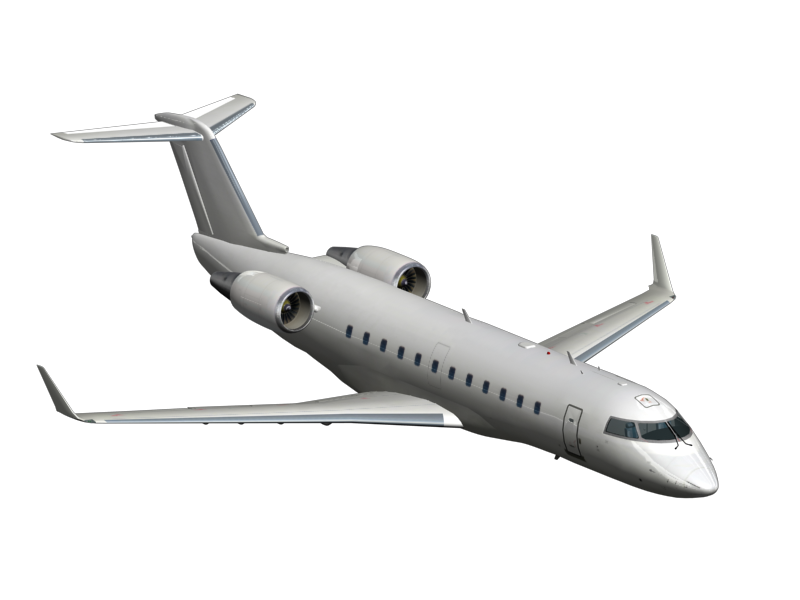
\includegraphics[width=\linewidth]{Figures/Bombardier_CRJ200}
  \end{minipage}%
  \begin{minipage}[b]{0.30\linewidth}
    \centering
    \begin{tabular}[b]{lll}
      \toprule
        \multicolumn{3}{c}{Legend} \\
      \midrule
        A & B & C \\
        0 & 0 & 0 \\
        0 & 1 & 0 \\
        1 & 0 & 0 \\
        1 & 1 & 1 \\
      \bottomrule
    \end{tabular}
    \vspace{5em}
  \end{minipage}
\caption{Figure and table side-by-side.}
\label{fig:side_by_side}
\end{figure}

 % file "Thesis_Results.tex"
%\cleardoublepage

%%%%%%%%%%%%%%%%%%%%%%%%%%%%%%%%%%%%%%%%%%%%%%%%%%%%%%%%%%%%%%%%%%%%%%%%%
%                                                                      %
%     File: Thesis_Conclusions.tex                                     %
%     Tex Master: Thesis.tex                                           %
%                                                                      %
%     Author: Andre C. Marta                                           %
%     Last modified :  2 Jul 2015                                      %
%                                                                      %
%%%%%%%%%%%%%%%%%%%%%%%%%%%%%%%%%%%%%%%%%%%%%%%%%%%%%%%%%%%%%%%%%%%%%%%%

\chapter{Conclusions}
\label{chapter:conclusions}

Insert your chapter material here...


% ----------------------------------------------------------------------
\section{Achievements}
\label{section:achievements}

The major achievements of the present work...


% ----------------------------------------------------------------------
\section{Future Work}
\label{section:future}

A few ideas for future work...

 % file "Thesis_Conclusions.tex"
%\cleardoublepage

% ----------------------------------------------------------------------
%  Bibliography
% ----------------------------------------------------------------------

% Add entry in the table of contents as chapter
\phantomsection
\addcontentsline{toc}{chapter}{\bibname}

% Include all references in .bib file, even non-cited ones...
%\nocite{*} % this should be used carefully because it is not correct!

% Produces the bibliography section when processed by BibTeX
%
% Bibliography style
% > entries ordered alphabetically
%\bibliographystyle{plain}
% > unsorted with entries appearing in the order in which the citations appear.
%\bibliographystyle{unsrt}
% > entries ordered alphabetically, with first names and names of journals and months abbreviated
%\bibliographystyle{abbrv}
% > entries ordered alphabetically, with reference markers based on authors' initials and publication year
%\bibliographystyle{alpha}
%
% Replacement bibliography styles provided by 'natbib' package
% (plainnat.bst, abbrvnat.bst, unsrtnat.bst )
% > entries ordered alphabetically
%\bibliographystyle{plainnat}
% > unsorted with entries appearing in the order in which the citations appear.
%\bibliographystyle{unsrtnat}
% > entries ordered alphabetically, with first names and names of journals and months abbreviated
%\bibliographystyle{abbrvnat} % <<<<< SELECT IF USING REFERENCES BY AUTHOR/YEAR
% > entries ordered alphabetically, with reference markers based on authors' initials and publication year
%\bibliographystyle{alpha}
%
% Custom bibliography style adapted from 'natbib' package
%   (based on http://tex.stackexchange.com/questions/5053/is-it-possible-to-get-unsrt-abbrv-bibliography)
%   (unsrtnat.bst + abbrvnat.bst -> abbrvunsrtnat.bst)
%   (original files copied from:
%   http://tug.ctan.org/macros/latex/contrib/natbib/abbrvnat.bst
%   http://tug.ctan.org/macros/latex/contrib/natbib/unsrtnat.bst
% > unsorted with entries appearing in the order in which the citations appear, with first names and names of journals and months abbreviated.
\bibliographystyle{abbrvunsrtnat} % <<<<< SELECT IF USING REFERENCES BY NUMBER (CITATION ORDER)

% External bibliography database file in the BibTeX format
\bibliography{Thesis_bib_DB} % file "Thesis_bib_DB.bib"

%\cleardoublepage

% ----------------------------------------------------------------------
%  Appendix (optional)
%
%  CAUTION: 1) the main document (up to the conclusions) shall not exceed 80 pages
%           2) the document shall not exceed a total of 100 pages (per IST regulations)
% ----------------------------------------------------------------------
%\appendix

% add page number prefix according to apendix chapter (optional)
%\renewcommand{\thepage}{\thechapter.\arabic{page}}

% re-set arabic numbering (A.1,A.2,...) (optional, use only if chapter prefix is added)
%\setcounter{page}{1}

%%%%%%%%%%%%%%%%%%%%%%%%%%%%%%%%%%%%%%%%%%%%%%%%%%%%%%%%%%%%%%%%%%%%%%%%%
%                                                                      %
%     File: Thesis_Appendix_A.tex                                      %
%     Tex Master: Thesis.tex                                           %
%                                                                      %
%     Author: Andre C. Marta                                           %
%     Last modified :  2 Jul 2015                                      %
%                                                                      %
%%%%%%%%%%%%%%%%%%%%%%%%%%%%%%%%%%%%%%%%%%%%%%%%%%%%%%%%%%%%%%%%%%%%%%%%

\chapter{Vector calculus}
\label{chapter:appendixVectors}

In case an appendix if deemed necessary, the document cannot exceed a total of 100 pages...

Some definitions and vector identities are listed in the section below.

% ----------------------------------------------------------------------
\section{Vector identities}
\label{section:vectorIdentities}

\begin{equation}
	\nabla \times \left( \nabla \phi \right) = 0
	\label{eq:cross_nnp}
\end{equation}

\begin{equation}
	\nabla \cdot \left( \nabla \times {\bf u} \right) = 0
	\label{eq:dotCross_nnu}
\end{equation}

 % file "Thesis_Appendix_A.tex"
%\cleardoublepage

% re-set arabic numbering (B.1,B.2,...) (optional, use only if chapter prefix is added)
%\setcounter{page}{1}

%%%%%%%%%%%%%%%%%%%%%%%%%%%%%%%%%%%%%%%%%%%%%%%%%%%%%%%%%%%%%%%%%%%%%%%%%
%                                                                      %
%     File: Thesis_Appendix_B.tex                                      %
%     Tex Master: Thesis.tex                                           %
%                                                                      %
%     Author: Andre C. Marta                                           %
%     Last modified :  2 Jul 2015                                      %
%                                                                      %
%%%%%%%%%%%%%%%%%%%%%%%%%%%%%%%%%%%%%%%%%%%%%%%%%%%%%%%%%%%%%%%%%%%%%%%%

\chapter{Technical Datasheets}
\label{chapter:appendixDatasheets}

It is possible to add PDF files to the document, such as technical sheets of some equipment used in the work.

% ----------------------------------------------------------------------
\section{Some Datasheet}
\label{section:datasheet}

% See more options to include PDF files in
% http://mirror.unl.edu/ctan/macros/latex/contrib/pdfpages/pdfpages.pdf
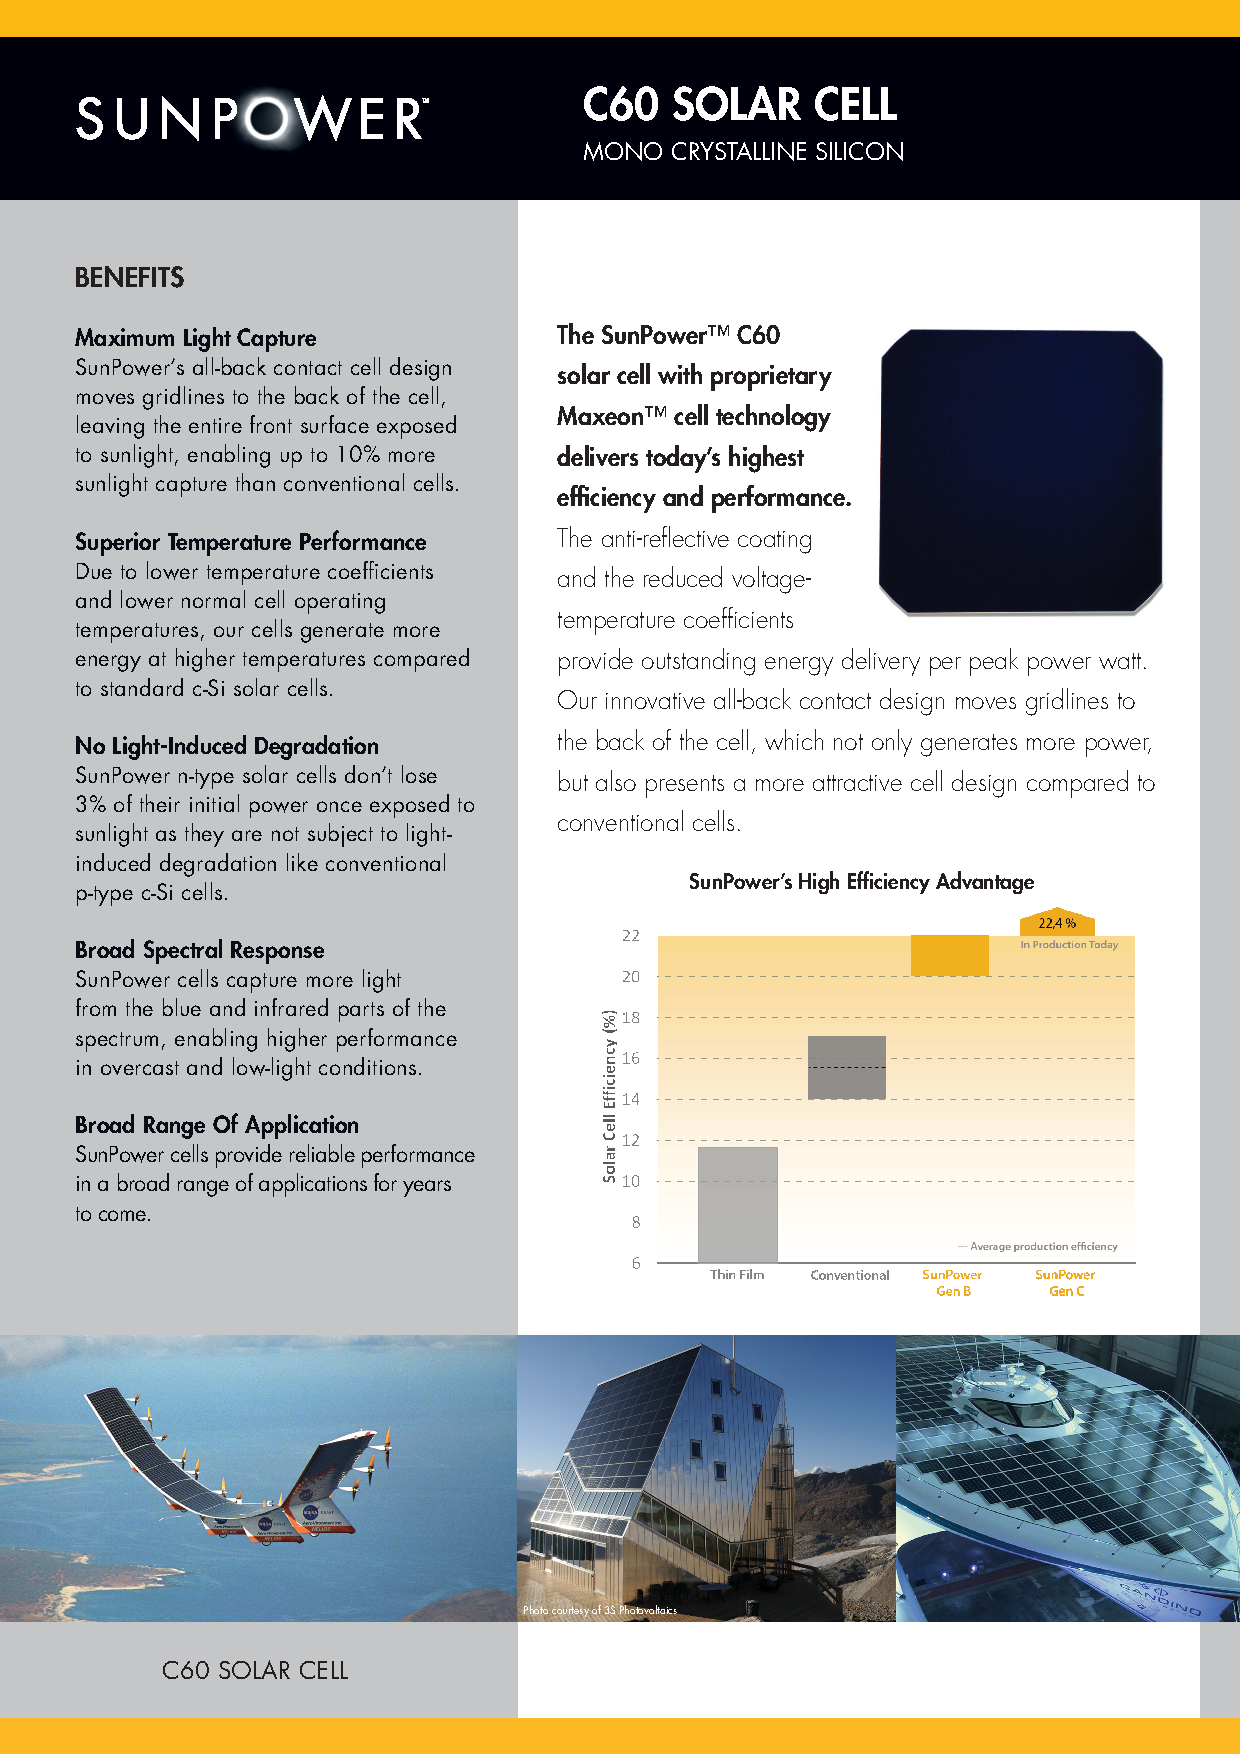
\includepdf[pages={1-2},nup=1x2,landscape=true]{Figures/SolarCell_Sunpower_C60.pdf}

 % file "Thesis_Appendix_B.tex"
%\cleardoublepage

% ----------------------------------------------------------------------
\end{document}
% ----------------------------------------------------------------------

